
% \subsection{Nonlinear Dynamics with Transition Noise }
% \label{subsec:nonlinear}

% To illustrate that our co-design approach works well for systems with \textbf{nonlinear} dynamics, we provide the following nonlinear
% example concerning an idealized mobile video streaming scenario. In this application, a mobile video client stores a buffer of video segments and must choose a video quality to download for the next segment of video. The goal is to maximize the quality of video while minimizing video stalls, which occur when the buffer under-flows while waiting for a segment to be downloaded. Here, state $x_t$ represents the buffer of stored video segments, control $u_t$ is segment quality, and $s_t$ is network throughput. The nonlinear dynamics are $x_{t+1} = [ x_{t} - u_t \oslash s_t ]_+ + L_x + \eta_{t}$, where $\oslash$ represents element-wise division, $L_x$ is the increase in stored video for each download, and $\eta_t$ is Gaussian transition noise. The cost aims to keep a positive buffer and have high video quality:
%     $\Jcontrol(\boldx, \boldu) = \sum_{t=0}^{T} \gamma_x \doublevert x_t - L_x \doublevert^2_2  + \sum_{t=0}^{T-1} \gamma_u \doublevert u_t - L_u\doublevert^2_2.$

% % \begin{figure}[ht]
% \vskip 0.2in
% \begin{center}
% \subfigure{
% {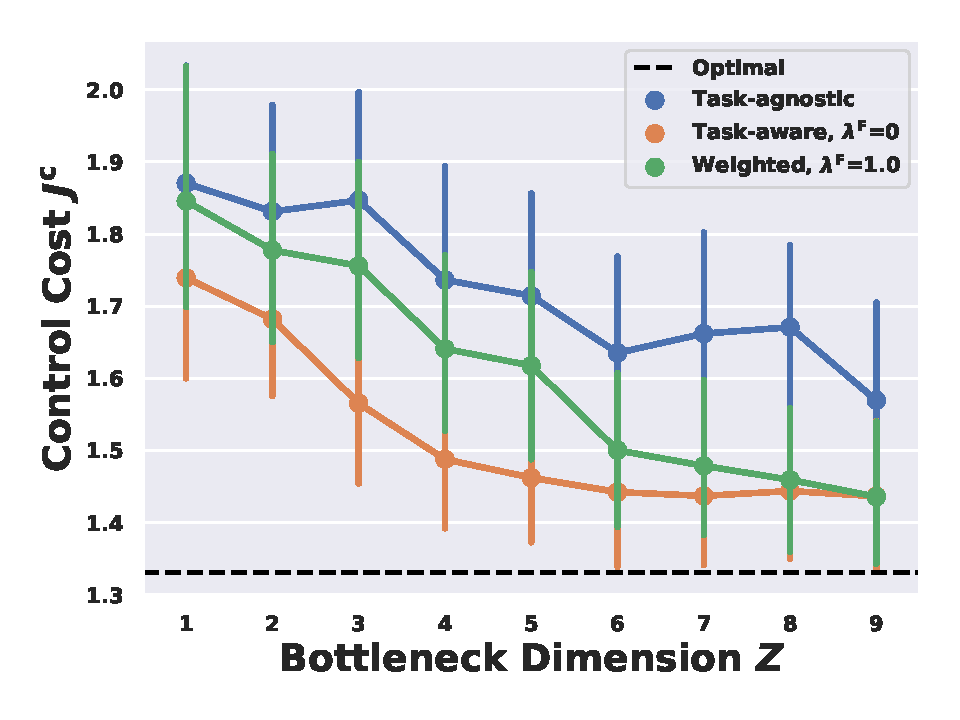
\includegraphics[width=0.6\columnwidth]{figures/video/video_cost_bottleneck.pdf}
% }}
% \caption{Co-Design Results with \textit{Nonlinear} Dynamics and Transition Noise.}
% \label{fig:nonlinear}
% \end{center}
% \vskip -0.2in
% \end{figure}

\begin{wrapfigure}{R}{0.5\columnwidth}
\centering
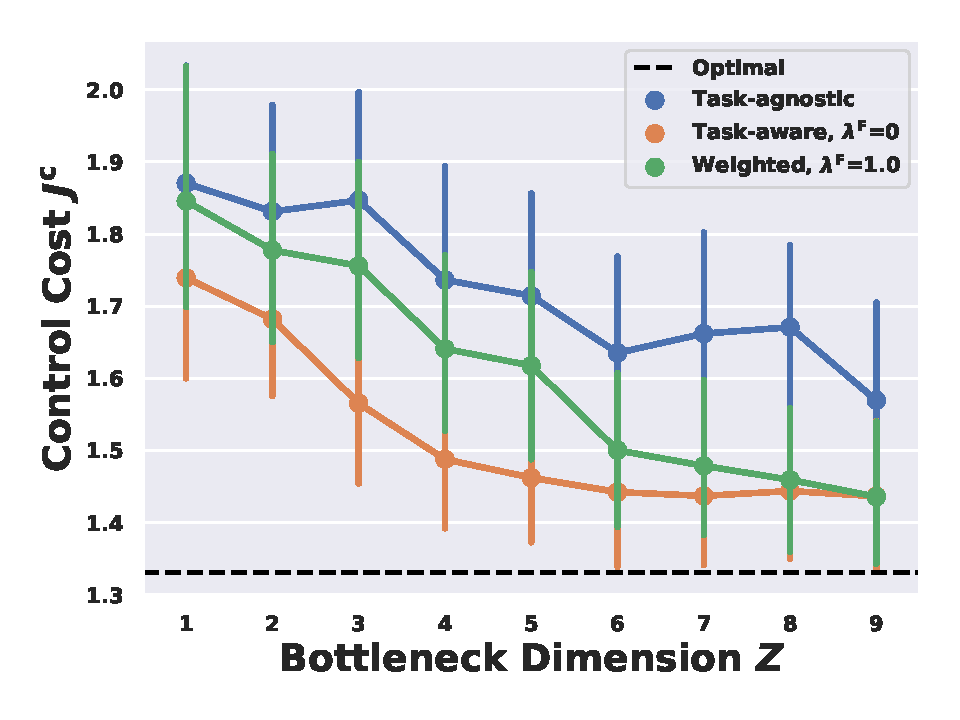
\includegraphics[width=0.5\columnwidth]{figures/video/video_cost_bottleneck.pdf}
\caption{Co-Design Results with \textit{Nonlinear} Dynamics and Transition Noise.}
\label{fig:nonlinear}
% \vskip -0.5em
\end{wrapfigure}

% Fig. \ref{fig:nonlinear} clearly shows our approach works quite well for a nonlinear scenario with transition noise, which complements the three diverse examples in the main paper. In the above experiments, the parameters are: $T=60$, $W = H = 15$, $m=n=p=4$, $\gamma_x = 0.25$, $\gamma_u = 1$, $L_x = 0.5 \times \mathbbm{1}_n$, $L_u = 0.2 \times \mathbbm{1}_m$. 

\subsection{Time Horizon} 
\begin{figure}[ht]
\vskip 0.2in
\begin{center}
\subfigure{
{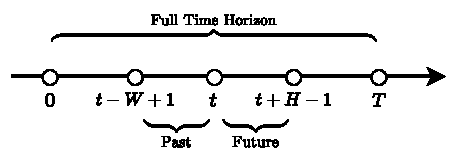
\includegraphics[width=0.6\columnwidth]{figures/time_horizon/time_horizon.pdf}}
}
\caption{Time horizon illustration.}
\label{fig:time_horizon}
\end{center}
\vskip -0.2in
\end{figure}

Fig. \ref{fig:time_horizon} illustrates the time horizon of the problem we consider in Sec. \ref{sec:problem_statement}.

\subsection{Input-driven LQR with Transition Noise} \label{subsec:lqr_transition_noise}
Suppose at each time interval $t$, we add a noise vector $w_t \in \reals^{n}$ with mean zero and covariance $\Sigma_{ww}$ to the dynamics:
\begin{align}
x_{t+1} = A x_t + B u_t + C s_t + w_t,
\end{align}
Then Eq. \ref{eq:rewrite_x_t} becomes
\begin{align}
    & x_{i+1} = A^{i+1} x_0 + \bm{M_{i}} \boldu + \bm{N_{i}} \bolds + \bm{P_i} \boldw
\end{align}
where $\boldw := w_{0:H-1}$ and $\bm{P_{i}} = \begin{bmatrix}
A^{i} & A^{i-1} & \cdots & I & \bm{0}
\end{bmatrix} \in \mathbb{R}^{n \times nH}$.

And hence Eq. \ref{eq:quadratic_jmpc} becomes
\begin{align}
\JMPC(\boldu; x_0, \bolds) ~=~ &  \boldu^\top (\underbrace{\bm{R} + \sum_{i=0}^{H-1} \bm{M_{i}}^\top Q \bm{M_{i}}}_{\bm{K}}) \boldu + 2[\underbrace{\sum_{i=0}^{H-1} \bm{M_{i}}^\top Q (A^{i+1} x_0 + \bm{N_{i}} \bolds + \bm{P_i} \boldw)}_{\bm{k}(x_0, \bolds)}]^\top \boldu + \\
& \underbrace{\sum_{i=0}^{H-1} (A^{i+1} x_0 + \bm{N_{i}} \bolds + \bm{P_i} \boldw)^\top Q (A^{i+1} x_0 + \bm{N_{i}} \bolds + \bm{P_i} \boldw)}_{\text{independent of $\boldu$}},
\end{align}
that is,
\begin{align}
\expec_\boldw[\JMPC(\boldu; x_0, \bolds)] ~=~ &  \boldu^\top (\underbrace{\bm{R} + \sum_{i=0}^{H-1} \bm{M_{i}}^\top Q \bm{M_{i}}}_{\bm{K}}) \boldu + 2[\underbrace{\sum_{i=0}^{H-1} \bm{M_{i}}^\top Q (A^{i+1} x_0 + \bm{N_{i}} \bolds)}_{\bm{k}(x_0, \bolds)}]^\top \boldu + \\
& \underbrace{\sum_{i=0}^{H-1} (A^{i+1} x_0 + \bm{N_{i}} \bolds)^\top Q (A^{i+1} x_0 +\bm{N_{i}} \bolds) + \expec_\boldw[(\bm{P_i} \boldw)^\top Q \bm{P_i} \boldw] }_{\text{independent of $\boldu$}}.
\end{align}

Notice that $\boldw$ only affects the constant term, which is independent of $\boldu$. Therefore, the analysis after Eq. \ref{eq:quadratic_jmpc} still holds.

% So $\boldu^*$ is independent of the noise $\boldw$ and the variance of $x_0$. $\JMPC$ is independent of $\E[x_0]$ but positively correlated to the variance of $x_0$.

% \subsection{Expectation of $x_0$}

% If the system is fully observable, then we know the exact the value of $x_0$, which will be $\E[x_0]$.

% If the system is not fully observable, then 
% $y_i = D x_i + v_i$

% Nee to find the estimate of $x_i$ with the smallest variation under the given observations. So
% $\E[x_{i+1}] = A \E[x_{i+1}] + B u_i + C s_i + L_i(y_i - D(A \E[x_{i+1}] + B u_i + C s_i))$
% where $L_i = AP_{i}D^\top(DP_iD^\top + \Sigma_{vv})^{-1}$ and 
% $P_{i+1} = A(P_i - P_i D^\top (D P_i D^\top + \Sigma_{vv})^{-1} DP_i)A^\top + \Sigma_{ww}$, and $P_0$ is the covariance matrix of $x_0$.

\subsection{Additional Explanations on the Proof of Proposition \ref{prop:input_dirven_lqr}}
Here, we provide some additional explanations on the proof of Proposition \ref{prop:input_dirven_lqr}, which are not included in the main paper due to space limits. 

1) \textbf{Positive definite matrix.} $\Psi + \lambdaforecast I$ ($\lambdaforecast > 0$) is positive definite because, $(\Psi + \lambdaforecast I)^\top = \Psi + \lambdaforecast I$, and $\Joverall \geq \lambdaforecast || \boldshat - \bolds||_2^2 > 0$ for any $\boldshat \neq \bolds$.

2) \textbf{Eigen-decomposition.}
The eigen-decomposition of $\Psi + \lambdaforecast I$ is $Y \Lambda Y^{-1}$, where $Y \in \reals^{\pH \times \pH}$ and the columns of $Y$ are the normalized eigen-vectors of $\Psi + \lambdaforecast I$, and $\Lambda \in \reals^{\pH \times \pH}$ is the diagonal matrix whose diagonal elements are the eigenvalues of $\Psi + \lambdaforecast I$. Since $\Psi + \lambdaforecast I$ is symmetric, $Y$ is also orthogonal, i.e., $Y^{-1} = Y^\top$. So $Y \Lambda Y^{-1} = Y \Lambda Y^\top$.

3) \textbf{Inverse matrix.} The matrix $\Lambda^{\frac{1}{2}}Y^\top$ is invertible because $\Psi + \lambdaforecast I$ is positive definite and its eigenvalues are all positive.

% 4) \textbf{Optimality.} If there is another encoder and decoder pair, denoted by ($E'$,$D'$), that achieves a smaller $\Joverall$ than ($E = \Omega Y^\top \Lambda^{\frac{1}{2}}$, $D = (Y^\top \Lambda^{\frac{1}{2}})^{-1}\Omega^\top $), then the projection $Y^\top \Lambda^{\frac{1}{2}})^{-1}E'$ and the inverse projection $Y^\top \Lambda^{\frac{1}{2}}D'$ give a solution to the PCA problem with smaller reconstruction error. This is contradictory to the assumption that $\Omega$ and $\Omega^\top$ are the optimal projection and inverse projection.

\subsection{Details on the LQR Simulations}

Here we provide further details on the two LQR simulations mentioned in Sec. \ref{subsec:input_driven_LQR}. In both of the simulations, vector timeseries $s$ has log, negative exponential, sine, square, and saw-tooth functions superimposed with a Gaussian random walk noise process.


\subsubsection{Basic LQR Simulation (Fig. \ref{fig:main_pca_full})}

\begin{figure*}[t]
\vskip 0.2in
\begin{center}


\includegraphics[width=0.8\columnwidth]{figures/pca_legend.pdf}

\subfigure{
{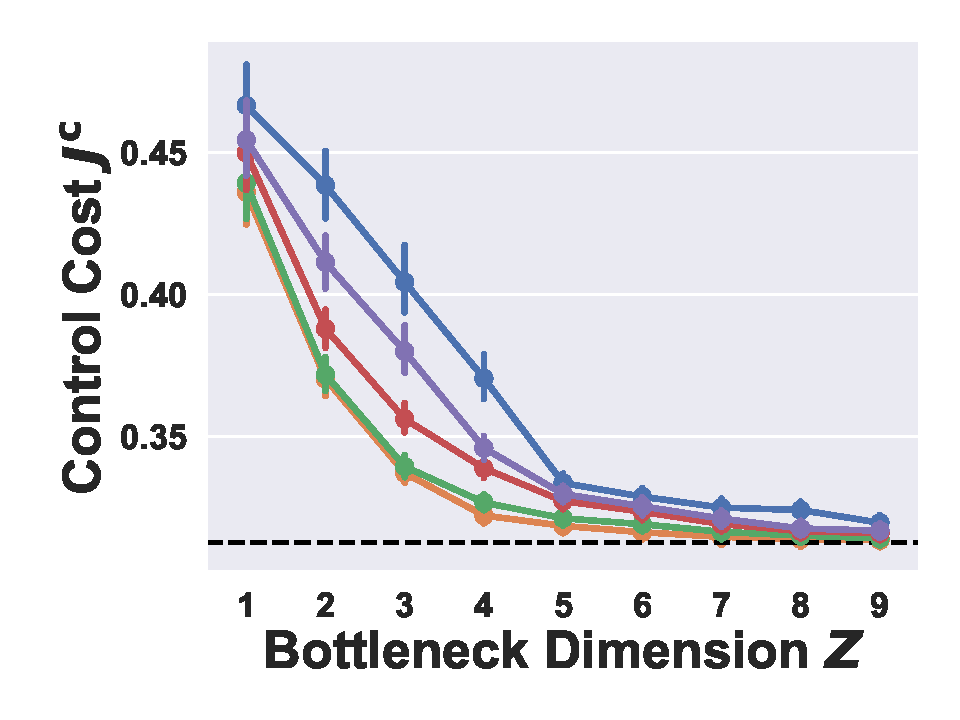
\includegraphics[width=0.4\columnwidth]{figures/pca_full/pca_full_cost_bottleneck.pdf}}
\label{fig_pca_full_cost_bottleneck}
}
\subfigure{
{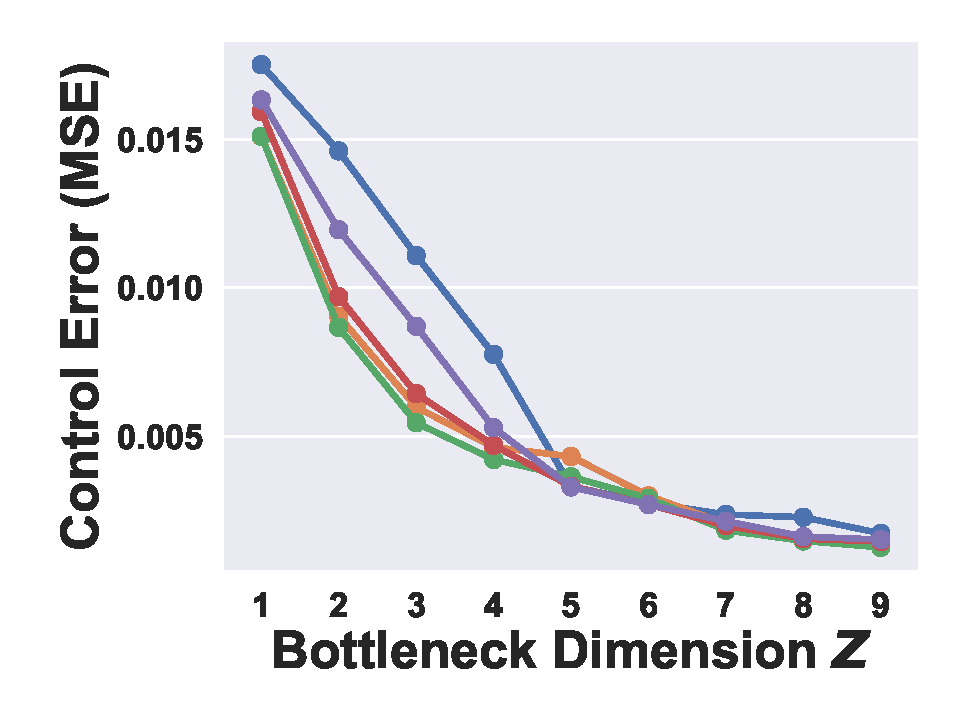
\includegraphics[width=0.4\columnwidth]{figures/pca_full/pca_full_ctrl_MSE.pdf}}
\label{fig_pca_full_ctrl_MSE}
}
\subfigure{
{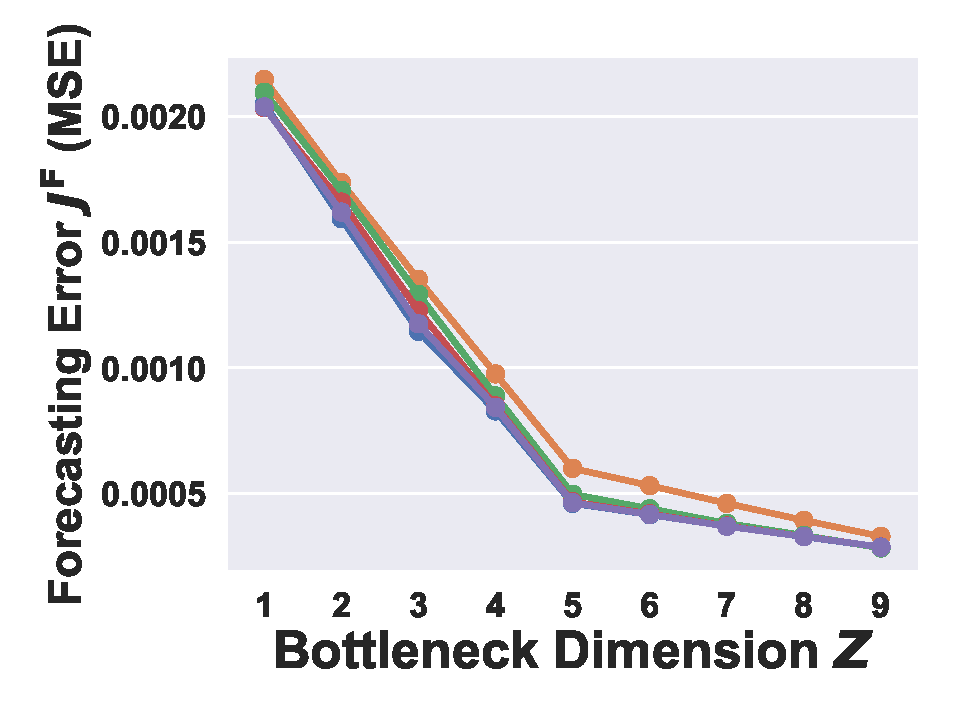
\includegraphics[width=0.4\columnwidth]{figures/pca_full/pca_full_fcst_MSE.pdf}}
\label{fig_pca_full_fcst_MSE}
}
\subfigure{
{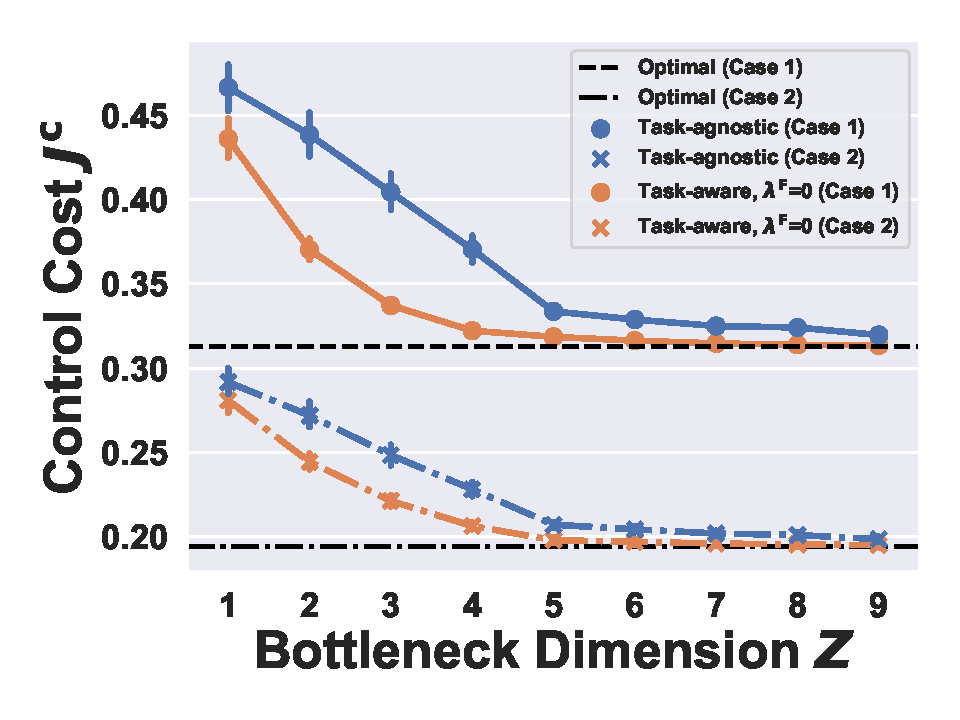
\includegraphics[width=0.4\columnwidth]{figures/pca_full/pca_cost_bottleneck_combined.pdf}
\label{fig_pca_full_forecast_errors}
}
}
\caption{\textbf{Analytic results for linear control:} (a) By only representing information salient to a control task, our co-design method (orange) achieves the optimal control cost with  
$43\%$
% $1.75\times$ 
less data than a standard MSE approach (``task-agnostic'', blue). Formal definitions of all benchmarks are in Sec. \ref{sec:evaluation}. (b-c) By weighting prediction error by $\lambdaforecast > 0$, we learn representations that are compressible, have good predictive power, and lead to near-optimal control cost (\eg~ $\lambdaforecast=1.0$).
(d) For the \textit{same} timeseries $\bolds$, two different control tasks require various amounts of data shared, motivating our task-centric representations.}
% \caption{\textbf{Analytic Results for Linear Control:} (a) By compressing information salient to a control task, our co-design method (orange) can effectively lower the control cost than a standard RMSE approach (``task-agnostic'', blue). Formal definitions of all benchmarks are in Sec. \ref{sec:evaluation}. (b-c) By weighting prediction error by $\lambdaforecast > 0$, we learn representations that are compressible, have good predictive power, and lead to near-optimal control cost (\eg $\lambdaforecast=1.0$).
% (d) For the \textit{same} timeseries $\bolds$ but a different control task (bottom), co-design method may not differ too much from the standard RMSE approach.}
\label{fig:main_pca_full}
\end{center}
\vskip -0.2in
\end{figure*}


1) \textbf{Dynamics:}
\begin{align*}
x_{t+1} = x_t + u_t - C s_t
\end{align*}
2) \textbf{Cost function:}
\begin{align*}
\JMPC = \frac{1}{1000} (\sum_{t=0}^{H} ||x_t||^2_2 + \sum_{t=0}^{H-1} ||u_t||^2_2) 
\end{align*}
3) \textbf{Parameters:} $H = 20$; $n = m = p = 5$; $C=\text{diag}(1, 2, \cdots, 5)$ for Fig. \ref{fig_pca_full_cost_bottleneck}-\ref{fig_pca_full_fcst_MSE} and Fig. \ref{fig_pca_full_forecast_errors} top, and $C=\text{diag}(1.5, 2, \cdots, 3.5)$ for Fig. \ref{fig_pca_full_forecast_errors} bottom.

As per Proposition \ref{prop:input_dirven_lqr}, we solve a simple low-rank approximation problem per bottleneck $Z$ to obtain the optimal encoder $E$, decoder $D$, and use Eqs. \ref{eq:low_rank_approximation}-\ref{eq:low_rank_approximation_final} to obtain the control and prediction costs. Clearly, our co-design algorithm (orange) outperforms a task-agnostic approach (blue) that simply optimizes for MSE.

\subsubsection{LQR Simulation with MPC (Fig. \ref{fig:main_pca})}
\begin{figure*}[t]
\vskip 0.2in
\begin{center}


\includegraphics[width=0.8\columnwidth]{figures/pca_legend.pdf}

\subfigure{
{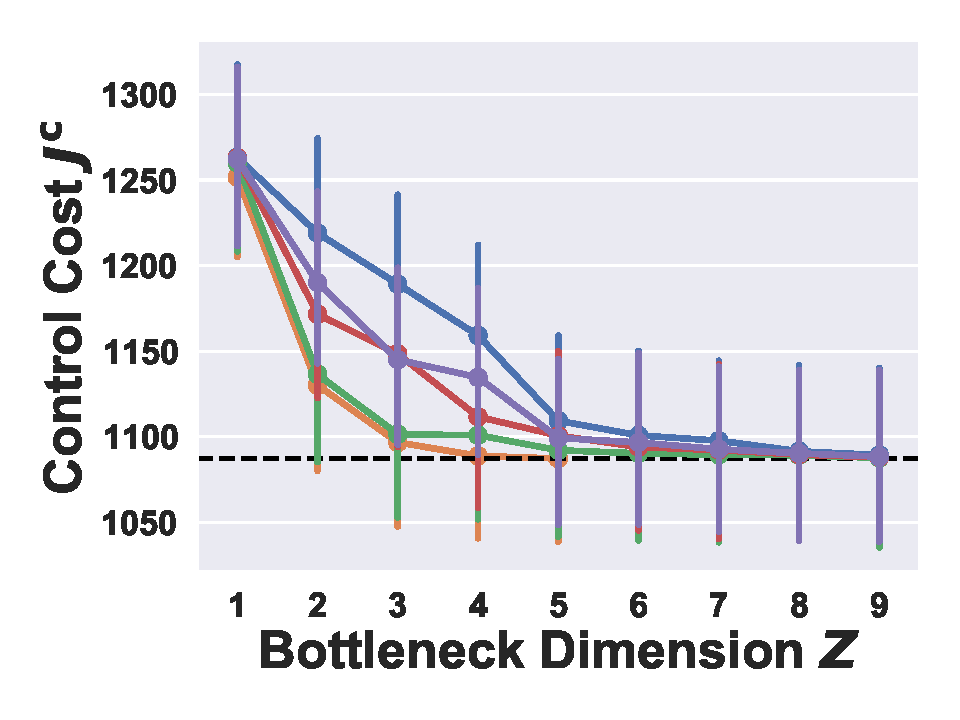
\includegraphics[width=0.4\columnwidth]{figures/pca/pca_mpc_cost_bottleneck.pdf}}
\label{fig_pca_cost_bottleneck}
}
\subfigure{
{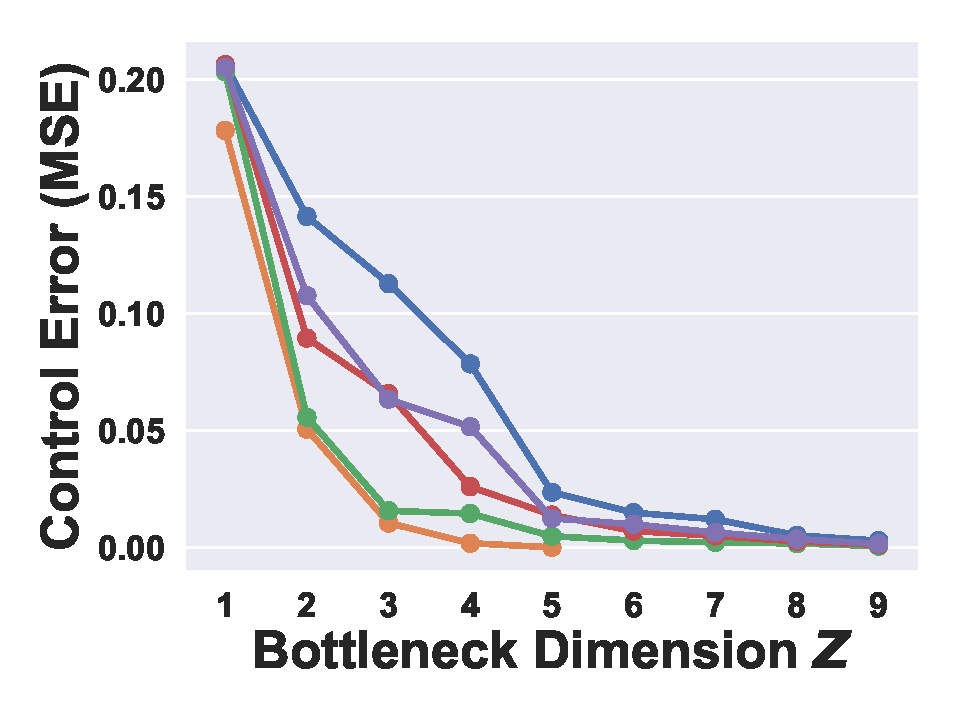
\includegraphics[width=0.4\columnwidth]{figures/pca/pca_mpc_ctrl_MSE.pdf}}
\label{fig_pca_ctrl_MSE}
}
\subfigure{
{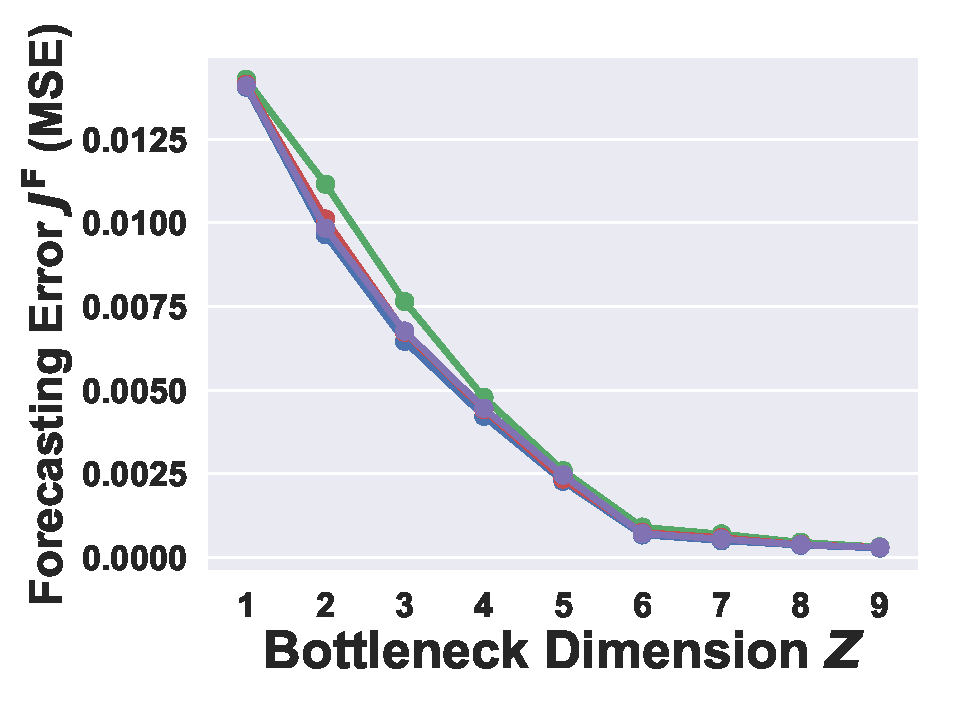
\includegraphics[width=0.4\columnwidth]{figures/pca/pca_mpc_fcst_MSE.pdf}}
\label{fig_pca_fcst_MSE}
}
\subfigure{
{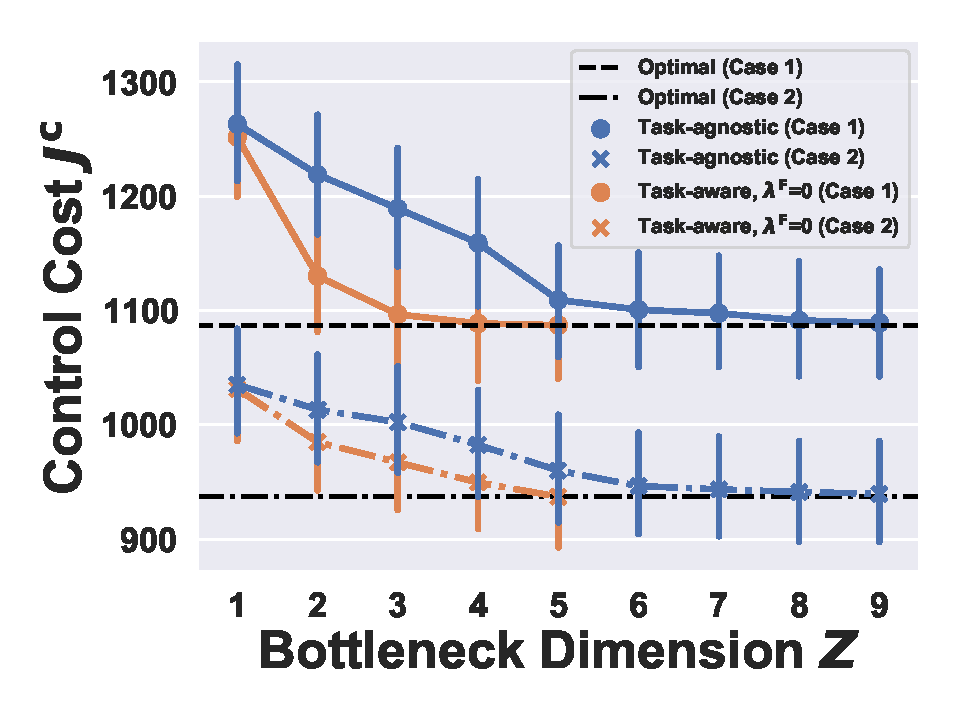
\includegraphics[width=0.4\columnwidth]{figures/pca/pca_cost_bottleneck_combined.pdf}
\label{fig_pca_forecast_errors}
}
}
\caption{\textbf{Linear control with MPC:} We repeat our analysis of input-driven LQR, but solve the problem in a receding horizon manner with forecasts for $H < T$ as discussed in Section \ref{subsec:input_driven_LQR} and Figure \ref{fig:main_pca_full}.
    (a) By only representing information salient to a control task, our co-design method (orange) achieves the optimal control cost with 
$60\%$ less data than a standard MSE approach (``task-agnostic'', blue). Formal definitions of all benchmarks are in Sec. \ref{sec:evaluation}. (b-c) By weighting prediction error by $\lambdaforecast > 0$, we learn representations that are compressible, have good predictive power, and lead to near-optimal control cost (\eg~ $\lambdaforecast=1.0$). The forecasting error of the task-aware scheme (orange) is much larger than the rest and thus not shown in the zoomed-in view.
(d) For the \textit{same} timeseries $\bolds$, two different control tasks require various amounts of data shared, motivating our task-centric representations.}
\label{fig:main_pca}
\end{center}
\vskip -0.2in
\end{figure*}


1) \textbf{Dynamics:}
\begin{align*}
x_{t+1} = x_t + u_t - C s_t
\end{align*}
2) \textbf{Cost function:}
\begin{align*}
\JMPC = \sum_{t=0}^{T} ||x_t||^2_2 + \sum_{t=0}^{T-1} ||u_t||^2_2 
\end{align*}
3) \textbf{Parameters:} $T = 100$, $W = H = 15$; $n = m = p = 5$; $C=\text{diag}(1, 2, \cdots, 5)$ for supplement Fig. \ref{fig_pca_cost_bottleneck}-\ref{fig_pca_fcst_MSE} and Fig. \ref{fig_pca_forecast_errors} top, and $C=\text{diag}(3, 3, \cdots, 3)$ for Fig. \ref{fig_pca_forecast_errors} bottom.

% We also run another LQR simulation with MPC, as shown in Fig. \ref{fig:main_pca}. The dynamics and the cost function are as follows:
% \begin{align*}
% & x_{t+1} = x_t + u_t - C s_t, \\
% & \JMPC = \sum_{t=0}^{T} ||x_t||^2_2 + \sum_{t=0}^{T-1} ||u_t||^2_2 
% \end{align*}

% The parameters are: 
% \begin{itemize}
% \item $T = 100$, $W = H = 15$, $n = m = p = 5$. 
% \item $C=\text{diag}(1, 2, \cdots, 5)$ for Fig. \ref{fig_pca_cost_bottleneck}-\ref{fig_pca_fcst_MSE} and Fig. \ref{fig_pca_forecast_errors} top; $C=\text{diag}(3, 3, \cdots, 3)$ for Fig. \ref{fig_pca_full_forecast_errors} bottom.
% \end{itemize}

% The data is the same as described in the last section.

\subsection{IoT Data Collection}
\begin{figure}[ht]
\vskip 0.2in
\begin{center}
\subfigure{
\raisebox{10mm}{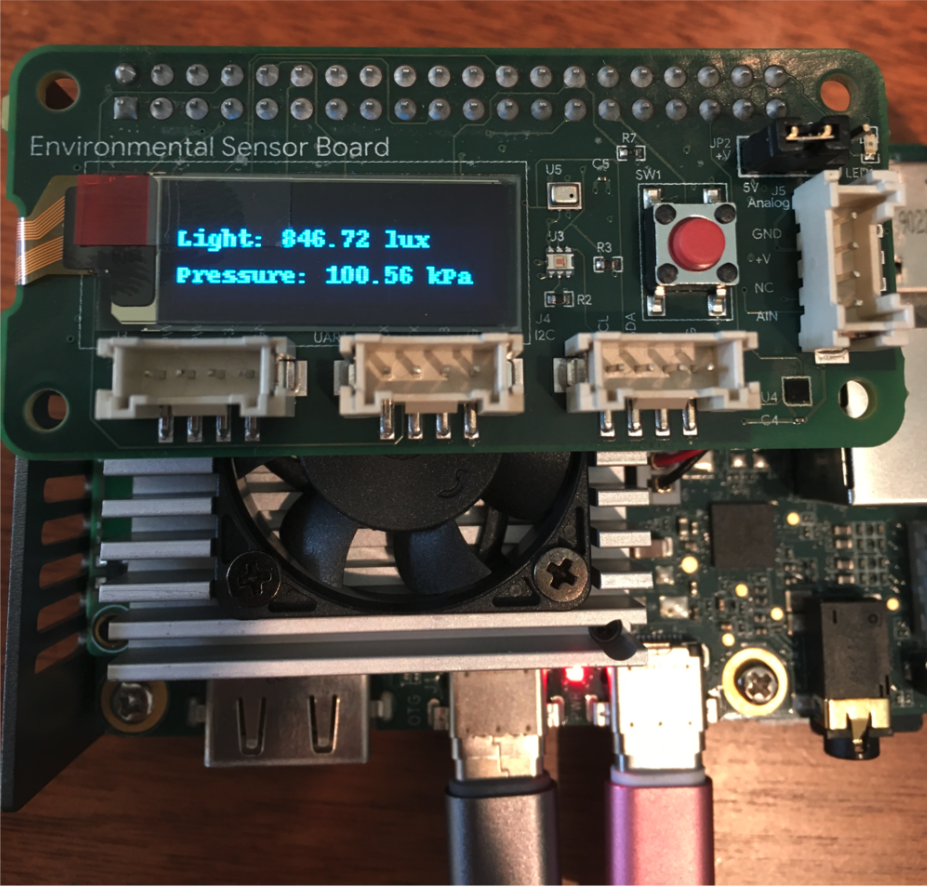
\includegraphics[width=0.2\columnwidth]{figures/appendix/iot/sensor/IoT_sensor.png}}
}
\subfigure{
{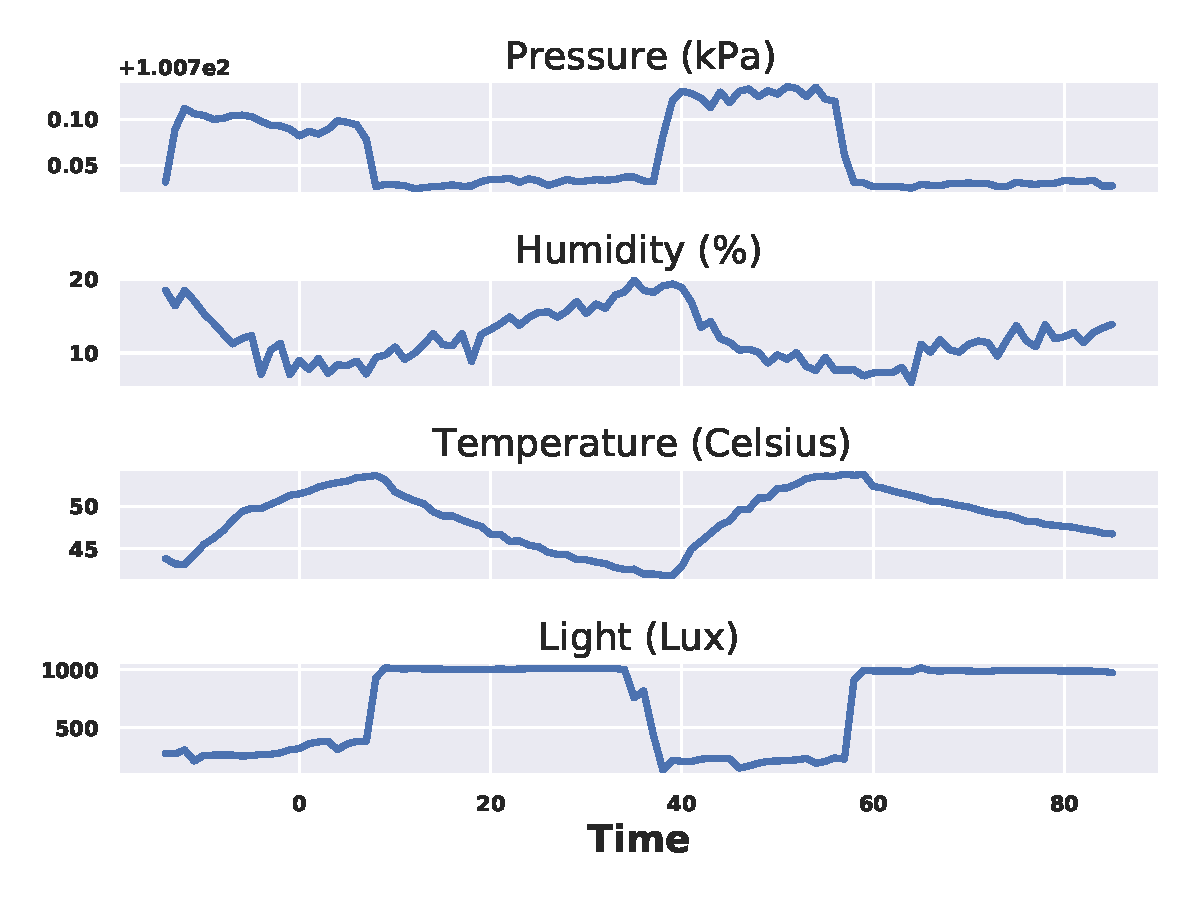
\includegraphics[width=0.6\columnwidth]{figures/appendix/iot/sensor/example_plot.pdf}}
}
\caption{Environmental sensor on the Google Edge TPU (left) and example stochastic timeseries (right).}
\label{fig:iot_sensor}
\end{center}
\vskip -0.2in
\end{figure}

Fig. \ref{fig:iot_sensor} shows the environmental sensor board (connected to an Edge TPU DNN accelerator) and an example of collected stochastic timeseries for our IoT data.

\subsection{Detailed Evaluation Settings}
\label{sec:appendix_evaluation}
\begin{figure}[ht]
\vskip 0.2in
\begin{center}
\centerline{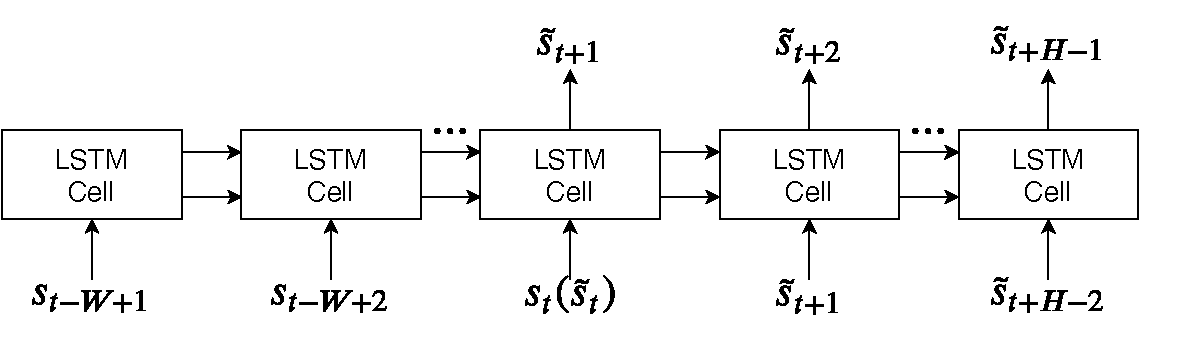
\includegraphics[width=0.8\columnwidth]{figures/appendix/model/lstm.pdf}}
\caption{LSTM timeseries network} 
\label{fig:lstm}
\end{center}
\vskip -0.2in
\end{figure}

\begin{figure}[ht]
\vskip 0.2in
\begin{center}
\centerline{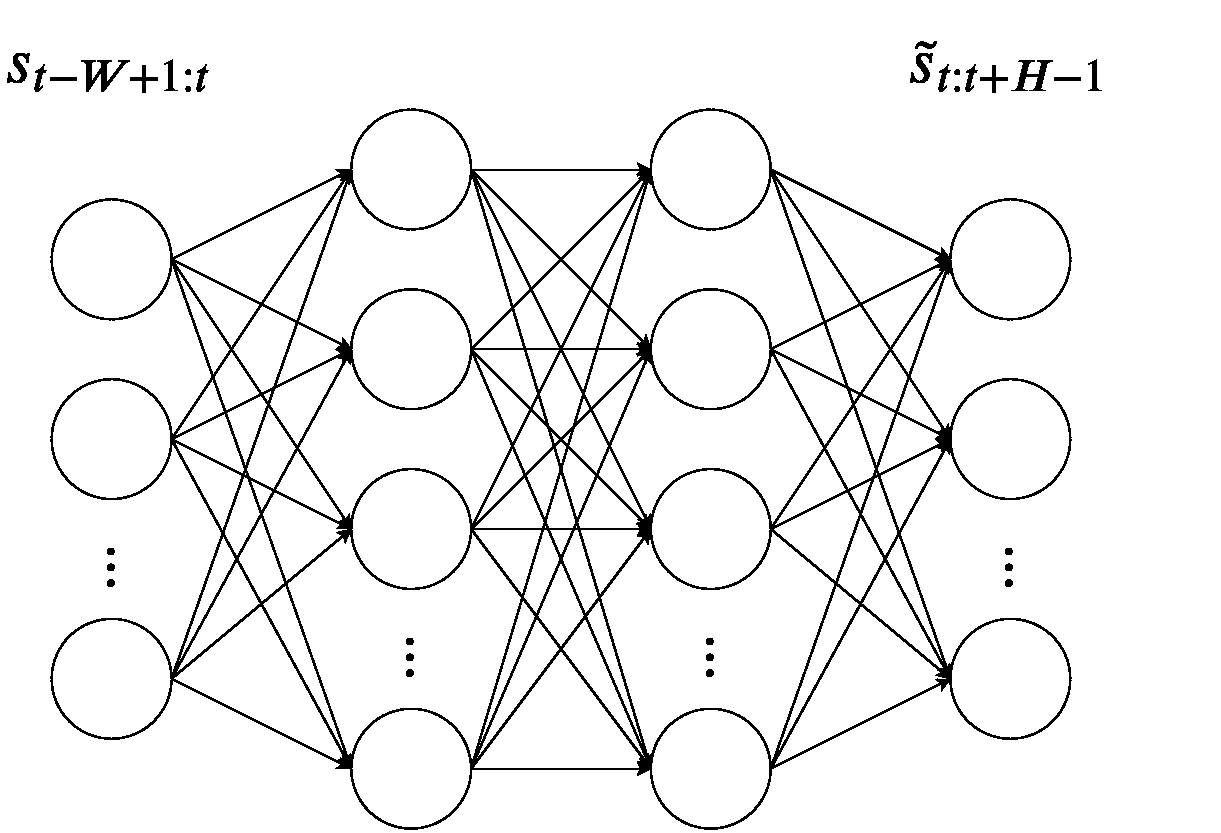
\includegraphics[width=0.5\columnwidth]{figures/appendix/model/DNN.pdf}}
\caption{2-hidden-layer feedforward network} 
\label{fig:DNN}
\end{center}
\vskip -0.2in
\end{figure}

We now provide further details on Sec. \ref{sec:evaluation} by summarizing the settings of our evaluation.

\subsubsection{Forecaster, Controller $\&$ Data Scaling}

\textbf{Basic Forecaster Settings.} In all three scenarios, the encoder parameters $\thetaencoder$ are responsible for \textit{both} forecasting and compression. We first have a forecasting model that first provides a full-dimensional forecast $\tilde{s}_{t:t+H-1}$, and then adopts simple linear encoder $E \in \reals^{\zbottleneck \times \pH}$ to yield $\phi_t$. The combination of the forecasting model's parameters and encoder $E$ constitute $\thetaencoder$. Then, a linear decoder $D \in \reals^{\pH \times \zbottleneck}$eventually produces decoded forecast $\hat{s}_{t:t+H-1}$. The model used to provide full-dimensional forecast $\tilde{s}_{t:t+H-1}$ varies case by case, as described subsequently.

\textbf{Smart Factory Regulation with IoT Sensors.} For forecasting, we adopt an LSTM timeseries network, as shown in Fig. \ref{fig:lstm}, with $W+H-2$ cells and hidden size $64$. The parameters associated with the forecaster and controller are set as follows: $T=72$, $W = H = 15$, $n = m = p = 4$; $u_\text{min} = -0.95 \times \mathbbm{1}_{p}, u_\text{max} = 0.95 \times \mathbbm{1}_{p}$, $\gamma_e = \gamma_s = \gamma_u = 1$. Further, we scale $s_t(i)$ to be within $[-1, 1], \forall i$.

\textbf{Taxi Dispatch Based on Cell Demand Data.} For forecasting, we adopt a 2-hidden-layer feedforward network, as shown in Fig. \ref{fig:DNN}, with hidden size $64$ and ReLu activation. The parameters associated with the forecaster and controller are set as follows: $T=32$, $W = H = 15$, $n = m = p = 4$; no constraint on $u_t$, and $\gamma_e = 1, \gamma_s = 100, \gamma_u = 1$. Further, we scale $s_t(i)$ to be within $[0, 1], \forall i$. 

\textbf{Battery Storage Optimization.} For forecasting, we adopt a 2-hidden-layer feedforward network, as shown in Fig. \ref{fig:DNN}, with hidden size $64$ and ReLu activation. The parameters associated with the forecaster and controller are set as follows: $T=122$, $W = H = 24$, $n = m = p = 8$; no constraint on $u_t$, and $\gamma_e = \gamma_s = \gamma_u = 1$. Further, we scale $s_t(i)$ to be within $[0, 1], \forall i$.

We observed similar performance for feedforward networks and LSTMs since the crux of our problem is to find a small set of task-relevant features for control.

\subsubsection{Training}
\begin{table}[ht]
\caption{Train/Test Timeseries, Training Epochs and Runtime.}
\label{tab:eval}
\vskip 0.15in
\begin{center}
\begin{small}
\begin{sc}
\begin{tabular}{lcccr}
\toprule
Dataset & Train/Test & Training & Runtime\\
& Timeseries & Epochs & \\
\midrule
IoT & 30/30 & 1000 & $<96$ hrs\\
Cell & 17/17 & 1000 & $<48$ hrs\\
Battery & 15/15 & 2000 & $<1$ hr \\
\bottomrule
\end{tabular}
\end{sc}
\end{small}
\end{center}
\vskip -0.1in
\end{table}

Our evaluation runs on a Linux machine with 4 NVIDIA GPUs installed (3 Geforce and 1 Titan).
Our code is based on Pytorch. We use the Adam optimizer and learning rate $10^{-3}$ for all the evaluations. The number of train/test timeseries\footnote{With MPC, each timeseries corresponds to $T$ samples, such as $T=72$ for the IoT scenario.}, training epochs, and resulting runtime are summarized in Table \ref{tab:eval}. 
The IoT dataset is provided in our code release and it does not have any personally identifiable or private information. 
% We provide our IoT dataset in our code release and will make it publicly-available (without any restrictions or license) online after the peer review process. The dataset does not have any personally identifiable or private information. 
The publicly-available electricity and cellular datasets did not have a stated license online. 


% \subsection{Key Result}
% \begin{table}[ht]
% \caption{Additional cost for each scheme on different datasets with the same compression gain -- the largest compression gain when task-aware scheme requires no more than $5\%$ additional cost.}
% \label{tab:key_result}
% \vskip 0.15in
% \begin{center}
% \begin{small}
% \begin{sc}
% \begin{tabular}{lcccr}
% \toprule
% Dataset & Task & Task & Weighted \\
% (Comp. gain) & Agnostic& Aware& \\
% \midrule
% IoT ($15\times$) & $32.3\%$ & $4.55\%$ & $7.30\%$ \\
% Cell ($15\times$) & $1435\%$ & $1.97\%$ & $41.6\%$ \\
% PJM ($96\times$) & $32.2\%$ & $4.38\%$ & $8.56\%$ \\
% \bottomrule
% \end{tabular}
% \end{sc}
% \end{small}
% \end{center}
% \vskip -0.1in
% \end{table}

% Table \ref{tab:key_result} presents the additional cost for each scheme on different datasets with the same compression gain. When the compression gains on the IoT, Cell and PJM dataset are $15\times$, $15\times$ and $96\times$ respectively, task-aware scheme requires only no more than $5\%$ additional cost, while task-agnostic scheme yields at least $30\%$ of the additional cost (notably, $1435\%$ additional cost on the cell dataset). Our weighted scheme yields a additional cost larger than the task-aware scheme but still relatively much smaller than the task-agnostic scheme. 

\subsection{Further Analysis on the Evaluation Results}
For better understanding of the differences between different schemes, we give further analysis on our evaluation results in Sec. \ref{sec:evaluation}.

\begin{figure*}[t]
\vskip 0.2in
\begin{center}
%\subfigure[]{
\subfigure{
{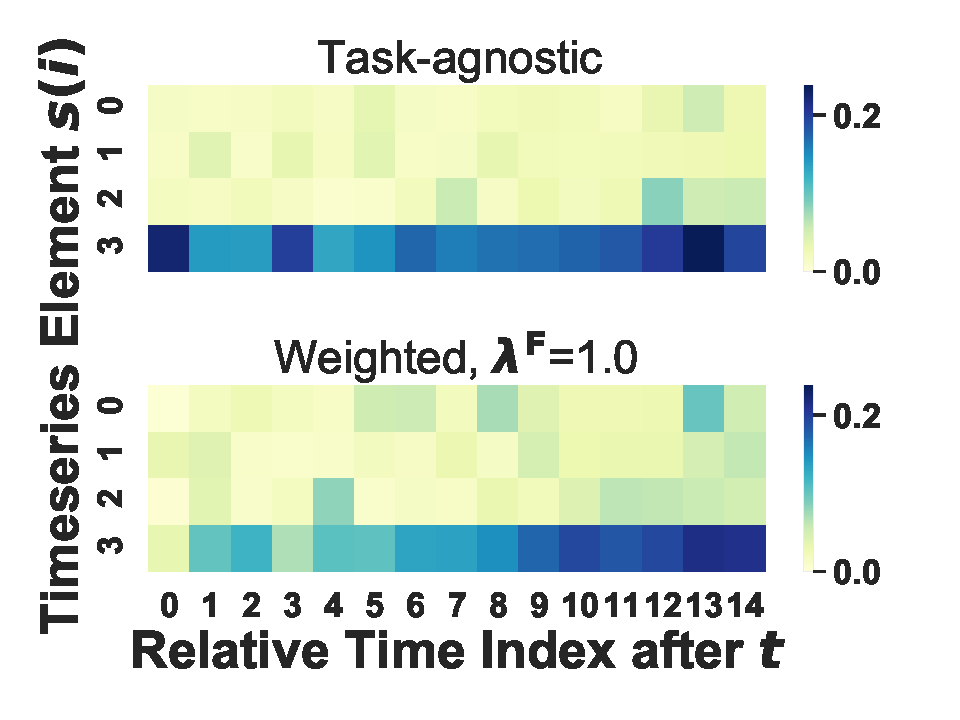
\includegraphics[width=0.31\columnwidth]{figures/iot/forecast_errors.pdf}}
\label{fig_iot_forecast_errors}
}
%\subfigure[]{
\subfigure{
{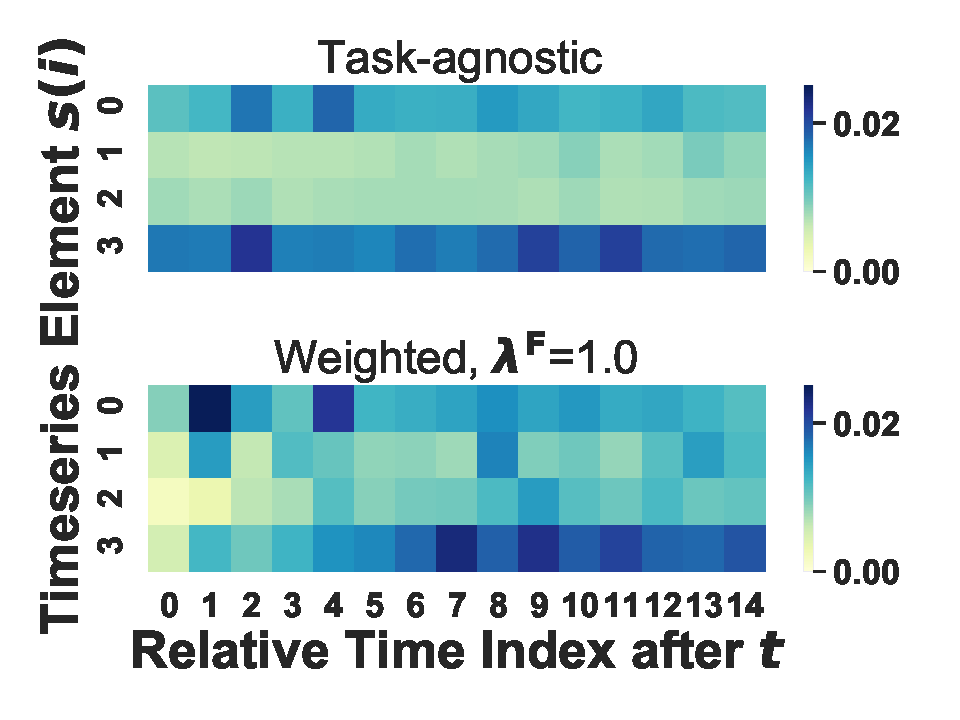
\includegraphics[width=0.31\columnwidth]{figures/cell/forecast_errors.pdf}}
\label{fig_cell_forecast_errors}
}
%\subfigure[]{
\subfigure{
{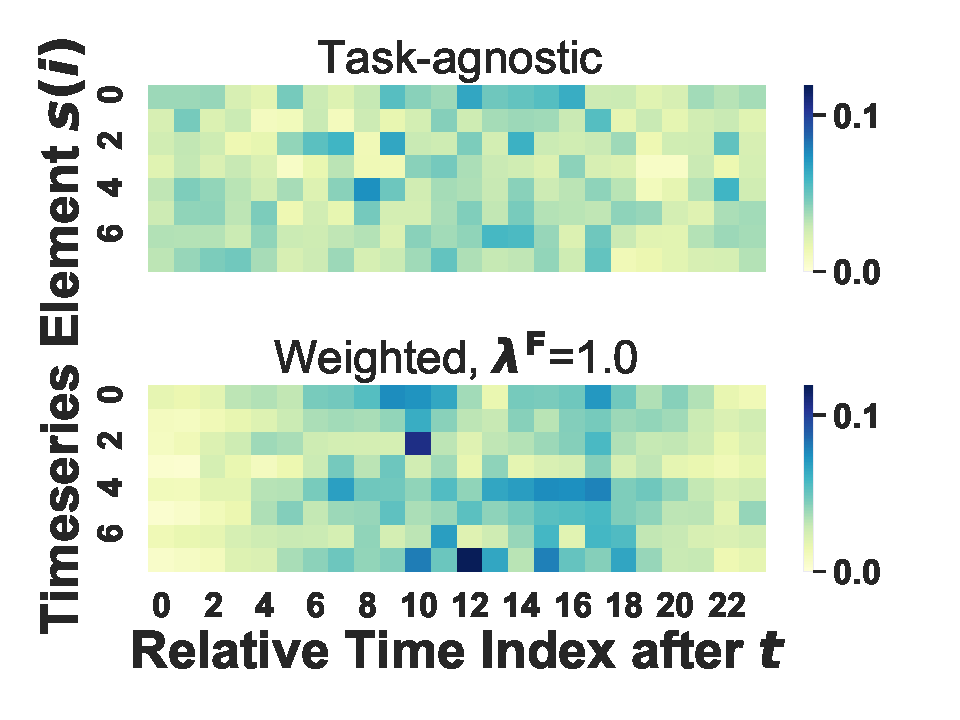
\includegraphics[width=0.31\columnwidth]{figures/pjm/forecast_errors.pdf}}
\label{fig_pjm_forecast_errors}
}
\caption{\textbf{Forecasting error comparison: task-agnostic vs. weighted scheme.} From left to right, the columns correspond to smart factory regulation from IoT sensors, taxi dispatching with cell demand, and battery storage optimization. The heatmaps show how co-design minimizes errors on timeseries elements $s(i)$ and forecast horizons that are salient for the control task when $Z=3$.}
\label{fig_heatmap}
\end{center}
\vskip -0.2in
\end{figure*}
%Aggregated forecasting error for  each relative time index when $Z=3$, under different policies. (j-l) Forecasting error for each $s(i)$ and each relative time index when $Z=3$, under task-agnostic (top) and weighted (bottom) policy, respectively.
%\caption{Results for real data. Columns from left to right corresponds to smart home regulation, taxi dispatching and battery storage optimization, respectively. (a-c) Control cost $J$ under different bottleneck dimension $Z$ and training policies; (d-f) Control error for each $u(i)$ when $Z=3$ under different training policies; (g-i) Aggregated forecasting error for  each relative time index when $Z=3$, under different policies. (j-l) Forecasting error for each $s(i)$ and each relative time index when $Z=3$, under task-agnostic (top) and weighted (bottom) policy, respectively.}

\textbf{Why does co-design yield task-relevant forecasts? (Continued)}

We further contrast the prediction errors made by task-agnostic and co-design approaches in the heatmaps of Fig. \ref{fig_heatmap}. In each heatmap, the x-axis represents the future time horizon, while the y-axis represents forecasting errors across various dimensions of timeseries $s$, denoted by $s(i)$.  Clearly, a weighted approach significantly reduces prediction error for near time-horizons, which is most pronounced for the battery dataset.


\begin{figure}[ht]
\vskip 0.2in
\begin{center}

\includegraphics[width=0.8\columnwidth]{figures/forecast_legend.pdf}

\subfigure{
{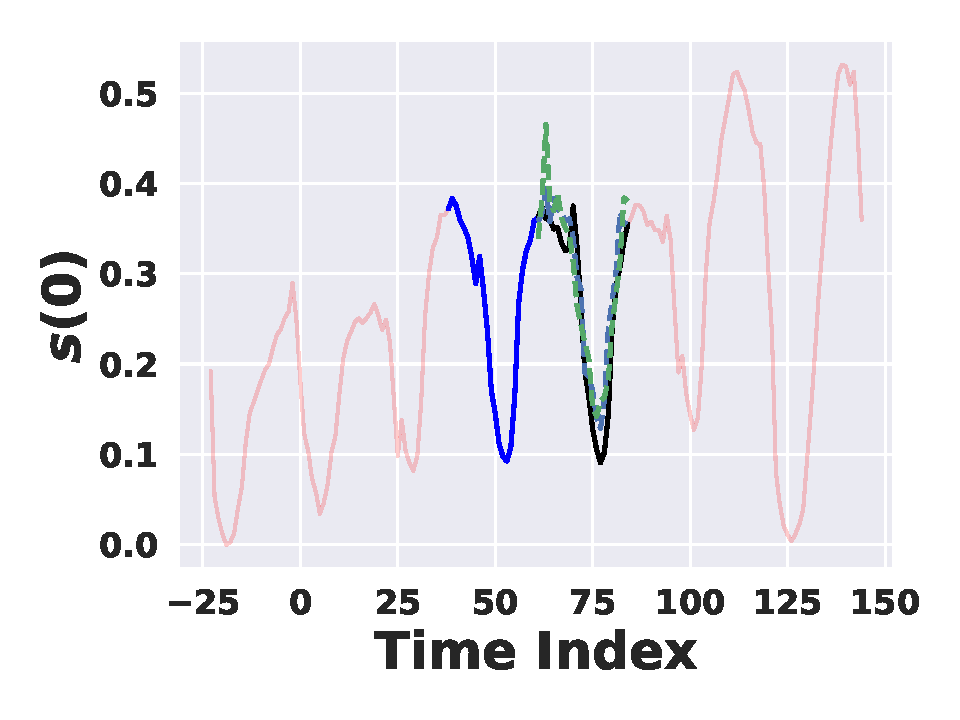
\includegraphics[width=0.4\columnwidth]{figures/appendix/pjm/z_9/forecasts_no_task_aware_sample_1_time_84_signal_0.pdf}}
}
\subfigure{
{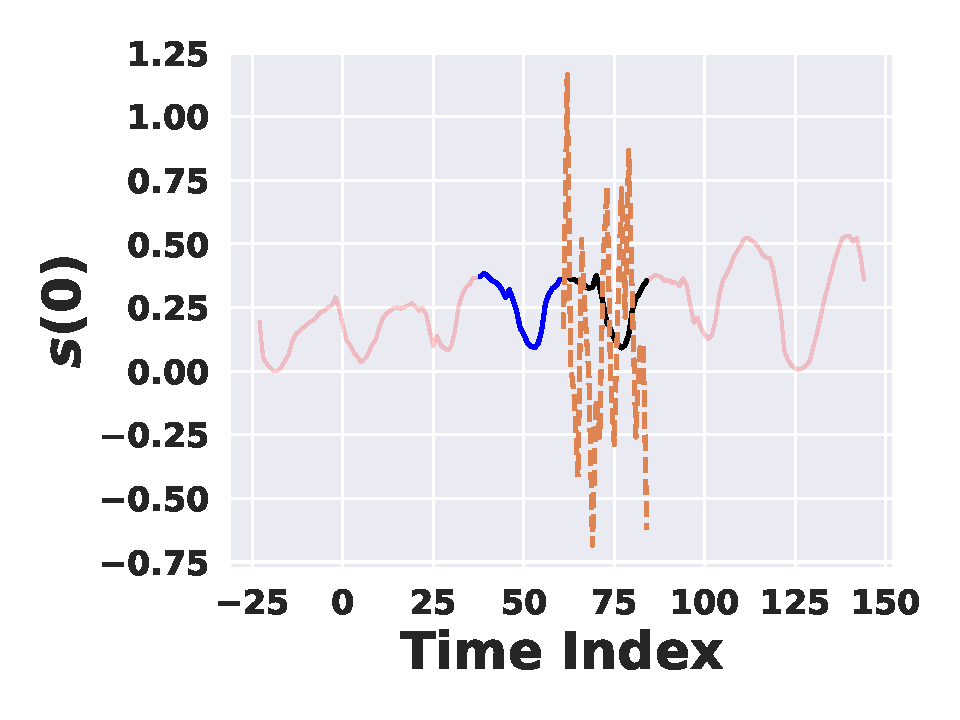
\includegraphics[width=0.4\columnwidth]{figures/appendix/pjm/z_9/forecasts_task_aware_sample_1_time_84_signal_0.pdf}}
}
\caption{\textbf{Forecast comparison: task-agnostic/weighted schemes vs. task-aware scheme.}  Example forecasts for the battery charging scenario at $t=84$ when $Z=9$, for both our task-agnostic/weighted schemes (left) and the task-aware scheme (right). Clearly, a fully task-aware approach with $\lambdaforecast = 0$ yields poor predictions since it does not regularize for prediction errors. This motivates our weighted co-design approach on the left.}
\label{fig:forecasts_comparison}
\end{center}
\vskip -0.2in
\end{figure}

\begin{figure}[ht]
\vskip 0.2in
\begin{center}


\includegraphics[width=0.8\columnwidth]{figures/forecast_legend_short.pdf}

\subfigure{
{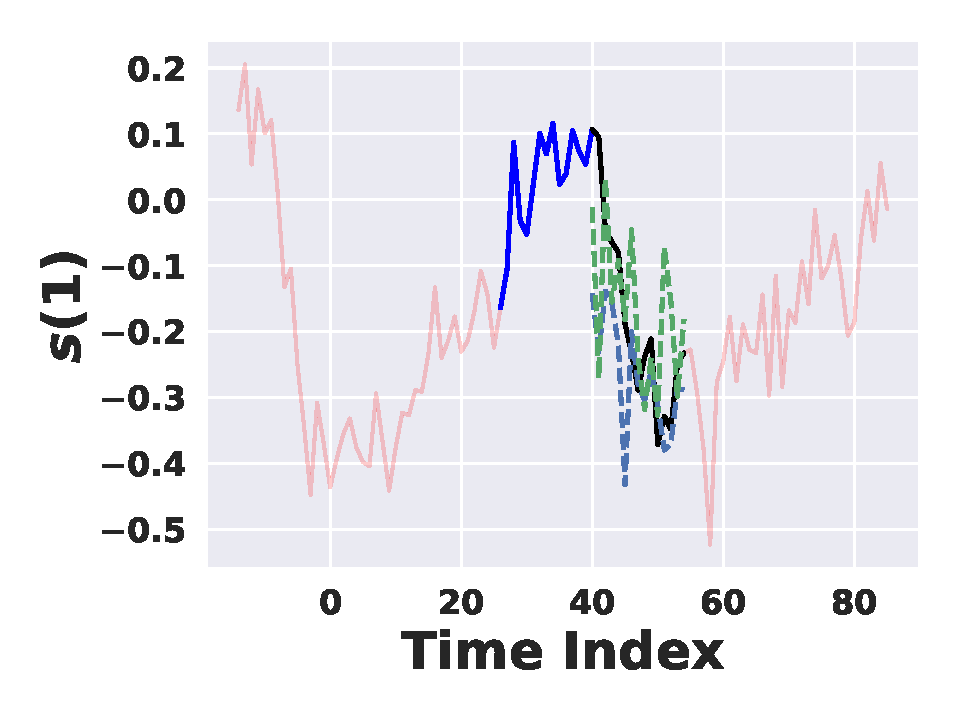
\includegraphics[width=0.4\columnwidth]{figures/appendix/iot/z_4/forecasts_no_task_aware_sample_15_time_54_signal_1.pdf}}
}
\subfigure{
{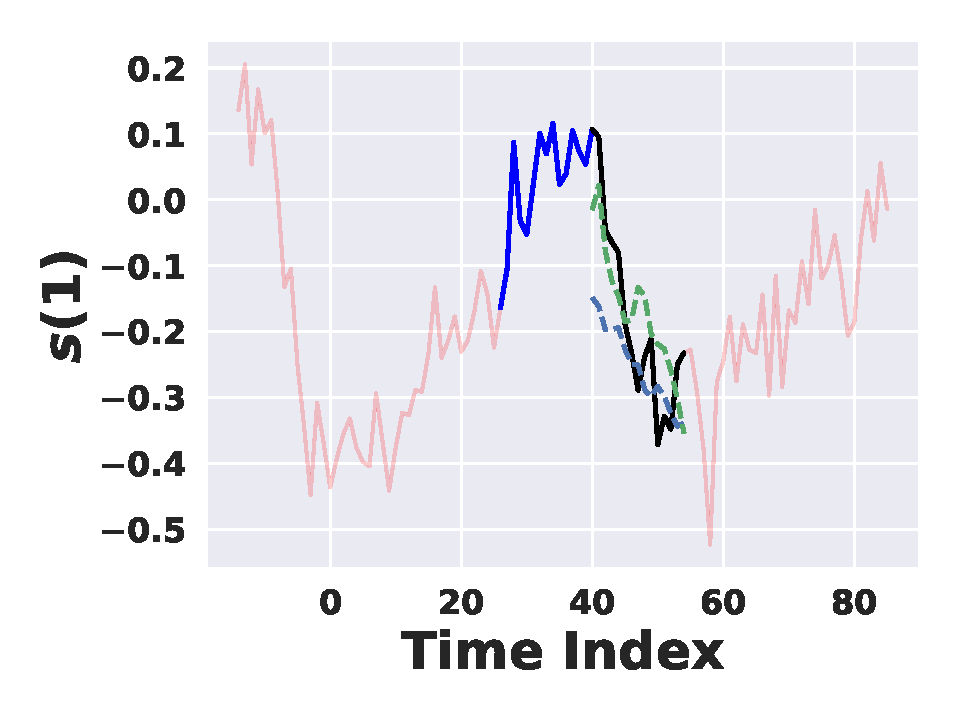
\includegraphics[width=0.4\columnwidth]{figures/appendix/iot/z_9/forecasts_no_task_aware_sample_15_time_54_signal_1.pdf}}
}
\subfigure{
{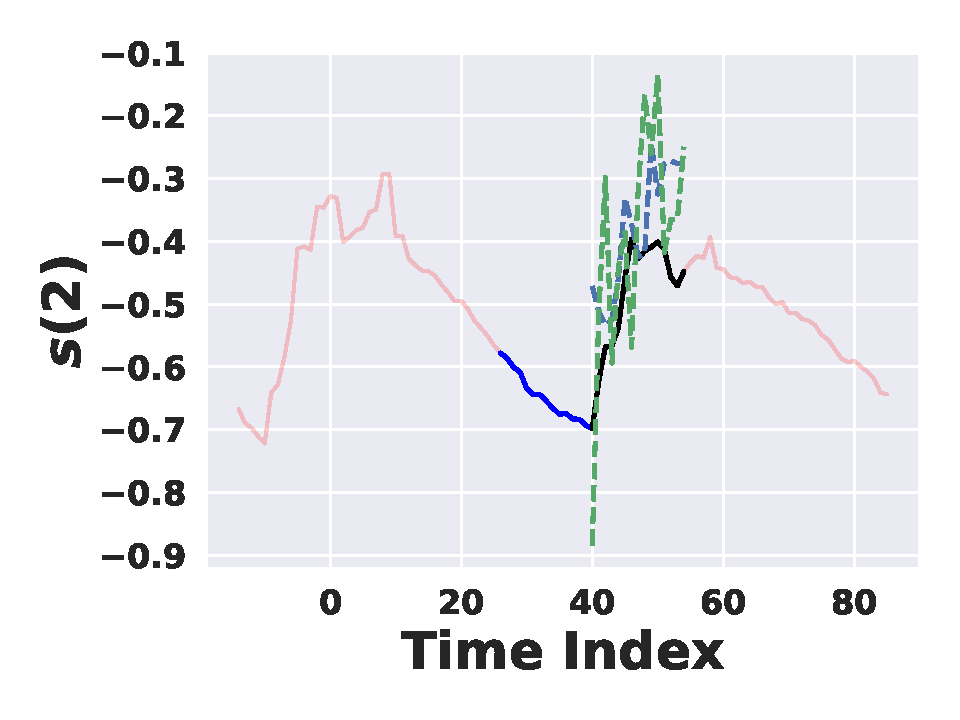
\includegraphics[width=0.4\columnwidth]{figures/appendix/iot/z_4/forecasts_no_task_aware_sample_15_time_54_signal_2.pdf}}
}
\subfigure{
{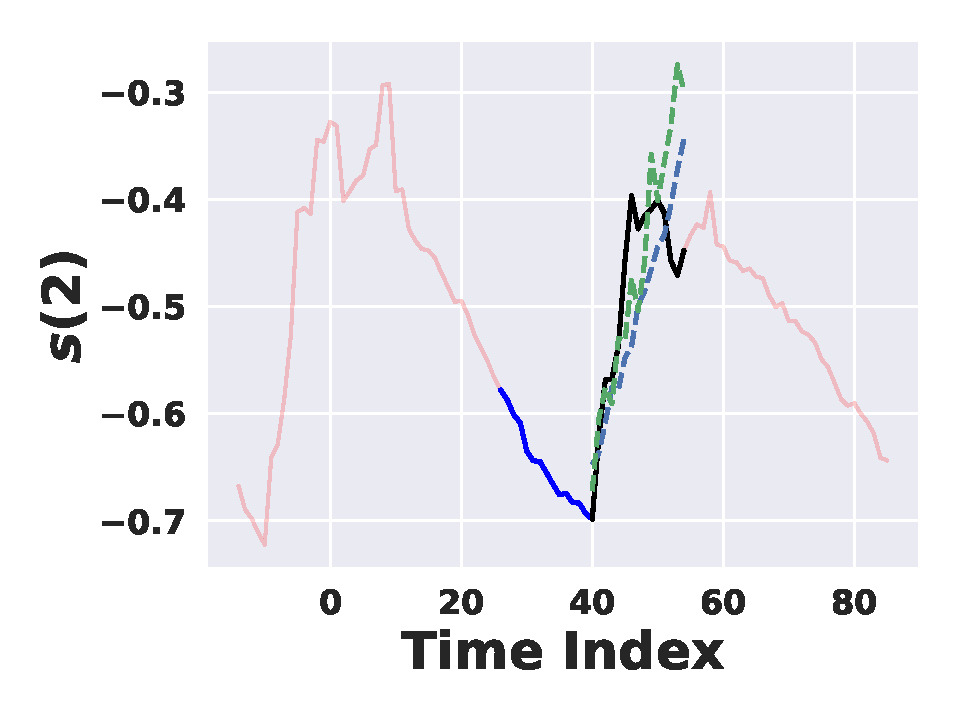
\includegraphics[width=0.4\columnwidth]{figures/appendix/iot/z_9/forecasts_no_task_aware_sample_15_time_54_signal_2.pdf}}
}

\caption{\textbf{Example forecasts (IoT sensors).}  Example forecasts at $t=40$ when $Z=4$ (left) and $Z=9$ (right). 
Clearly, the predictions are more accurate and smooth when $Z=9$. However, with a smaller bottleneck of $Z=4$ (left), we achieve near-optimal control performance since we capture task-relevant features with a coarse forecast that captures high-level, but salient, trends.}
\label{fig:iot_forecasts}
\end{center}
\vskip -0.2in
\end{figure}

\begin{figure}[ht]
\vskip 0.2in
\begin{center}


\includegraphics[width=0.8\columnwidth]{figures/forecast_legend_short.pdf}

\subfigure{
{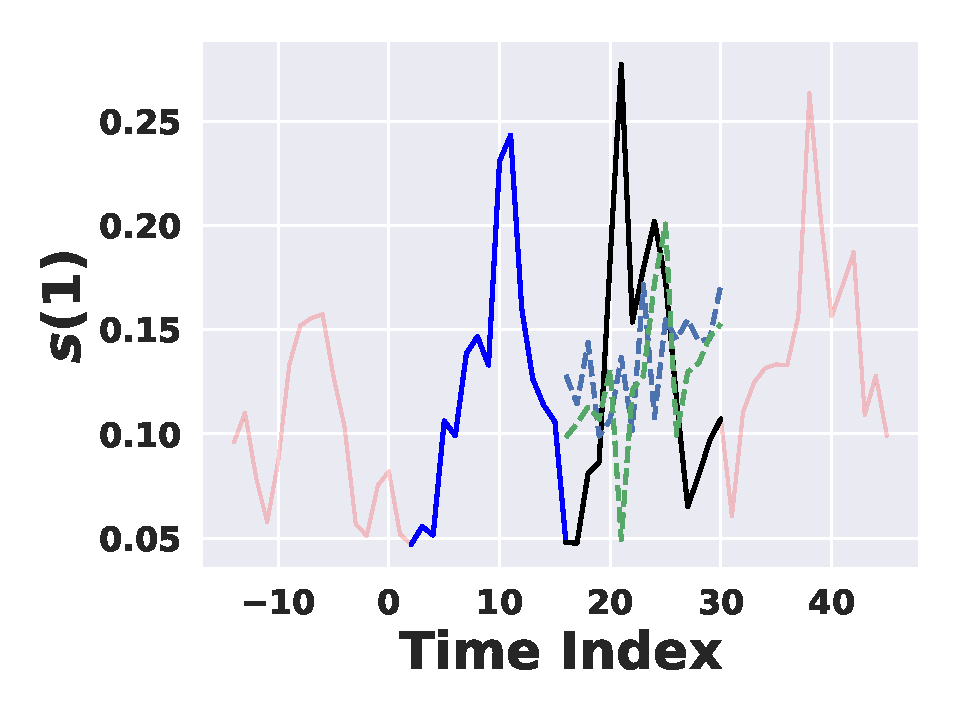
\includegraphics[width=0.4\columnwidth]{figures/appendix/cell/z_4/forecasts_no_task_aware_sample_1_time_30_signal_1.pdf}}
}
\subfigure{
{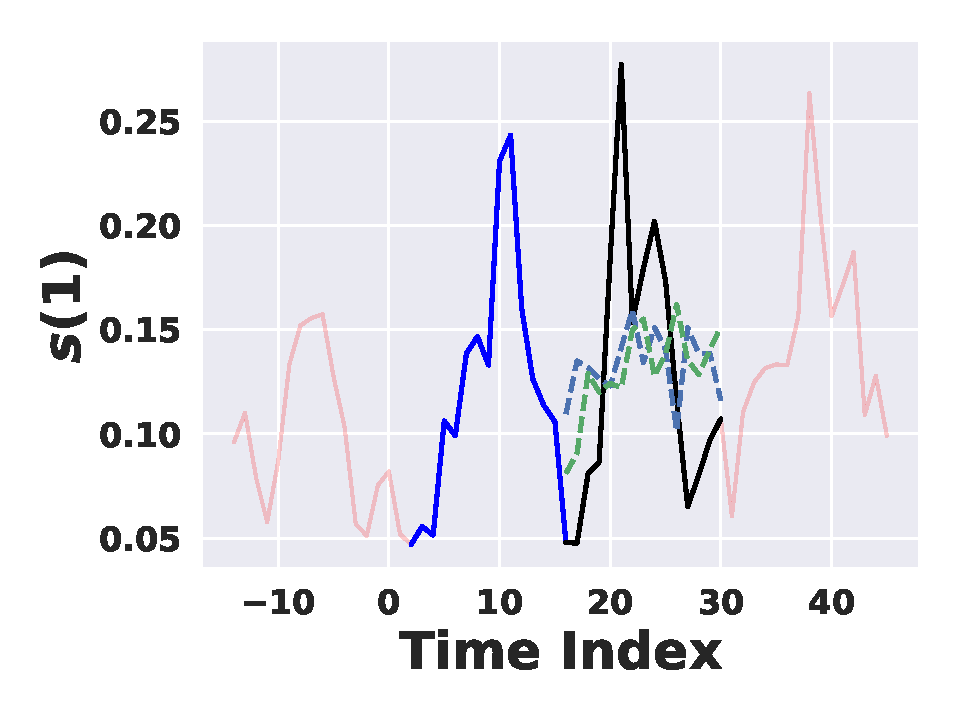
\includegraphics[width=0.4\columnwidth]{figures/appendix/cell/z_9/forecasts_no_task_aware_sample_1_time_30_signal_1.pdf}}
}

\subfigure{
{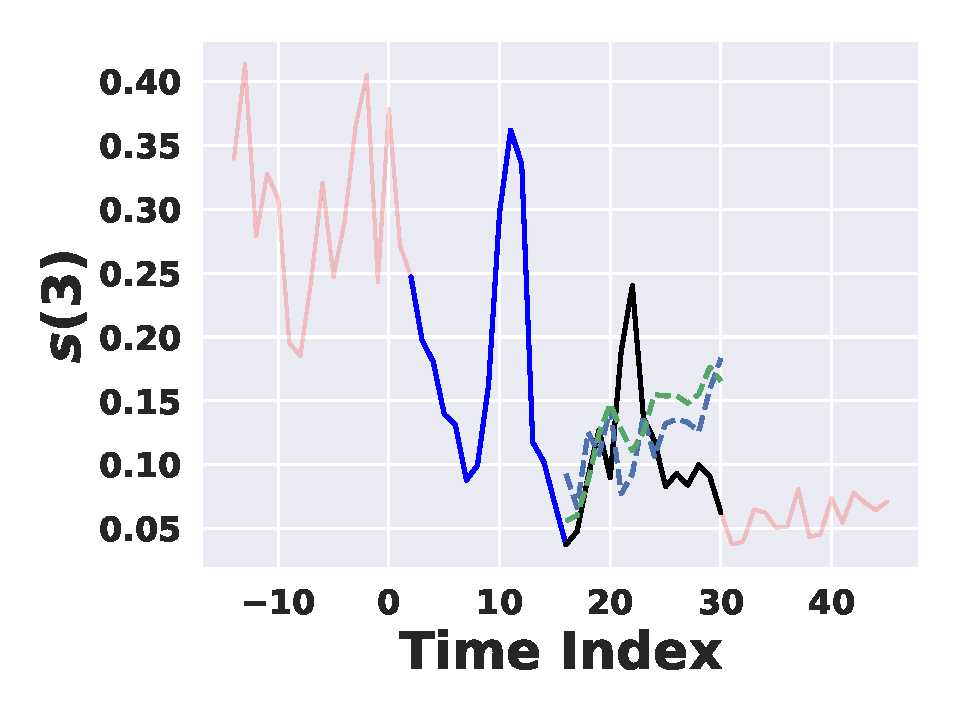
\includegraphics[width=0.4\columnwidth]{figures/appendix/cell/z_4/forecasts_no_task_aware_sample_1_time_30_signal_3.pdf}}
}
\subfigure{
{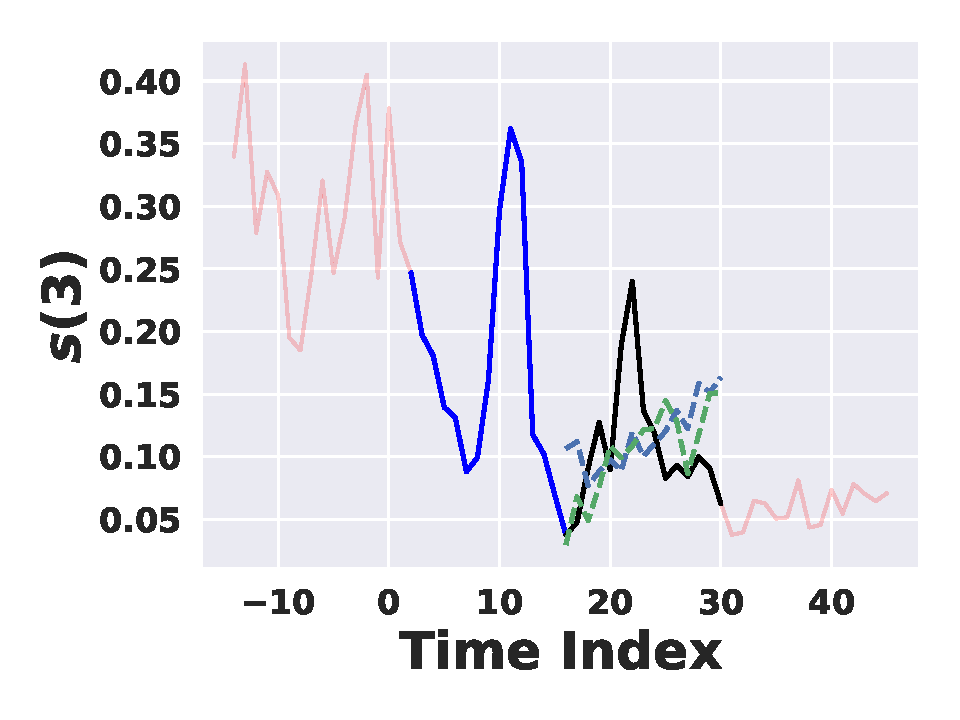
\includegraphics[width=0.4\columnwidth]{figures/appendix/cell/z_9/forecasts_no_task_aware_sample_1_time_30_signal_3.pdf}}
}


\caption{\textbf{Example forecasts (taxi scheduling).}  Example forecasts at of at $t=16$ when $Z=4$ (left) and $Z=9$ (right). This scenario had the worst prediction errors since the cell data is highly stochastic.}
\label{fig:cell_forecasts}
\end{center}
\vskip -0.2in
\end{figure}

\begin{figure}[ht]
\vskip 0.2in
\begin{center}


\includegraphics[width=0.8\columnwidth]{figures/forecast_legend_short.pdf}

\subfigure{
{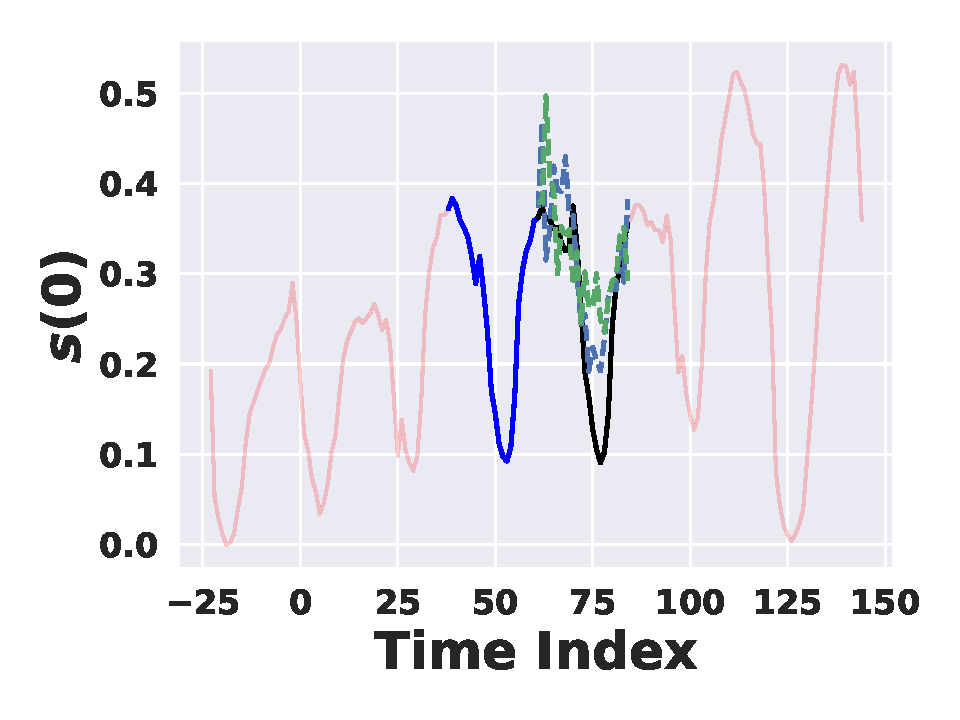
\includegraphics[width=0.4\columnwidth]{figures/appendix/pjm/z_4/forecasts_no_task_aware_sample_1_time_84_signal_0.pdf}}
}
\subfigure{
{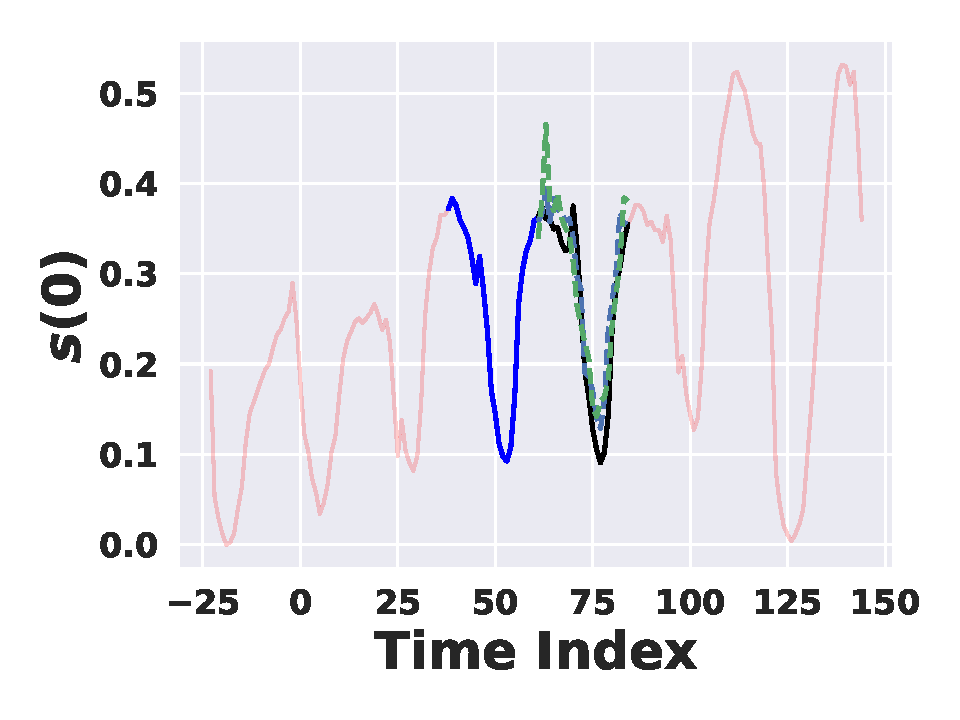
\includegraphics[width=0.4\columnwidth]{figures/appendix/pjm/z_9/forecasts_no_task_aware_sample_1_time_84_signal_0.pdf}}
}
\subfigure{
{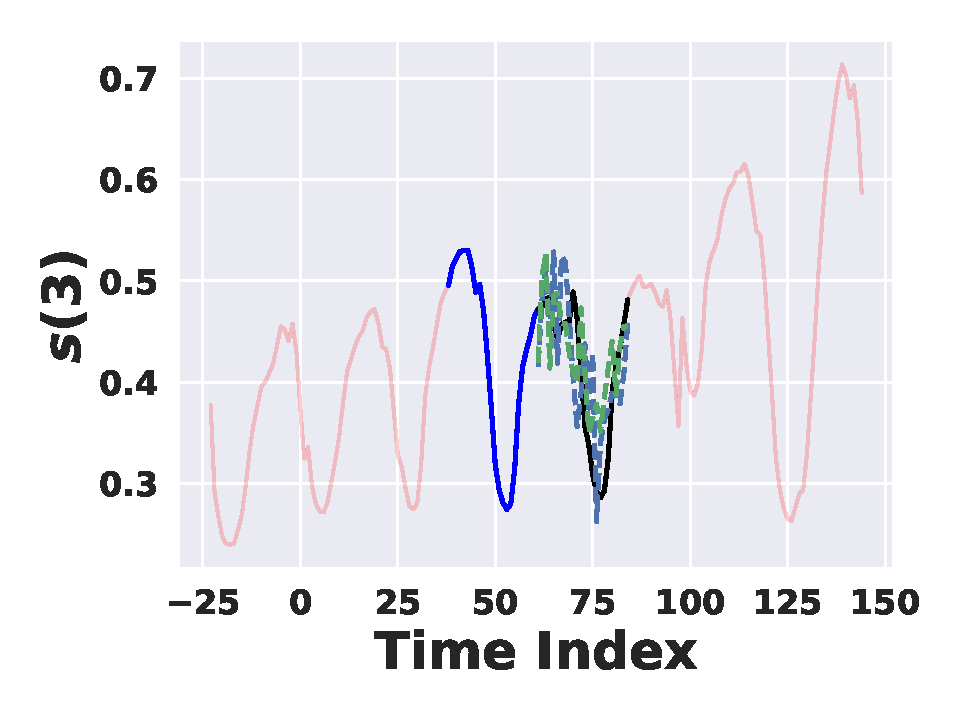
\includegraphics[width=0.4\columnwidth]{figures/appendix/pjm/z_4/forecasts_no_task_aware_sample_1_time_84_signal_3.pdf}}
}
\subfigure{
{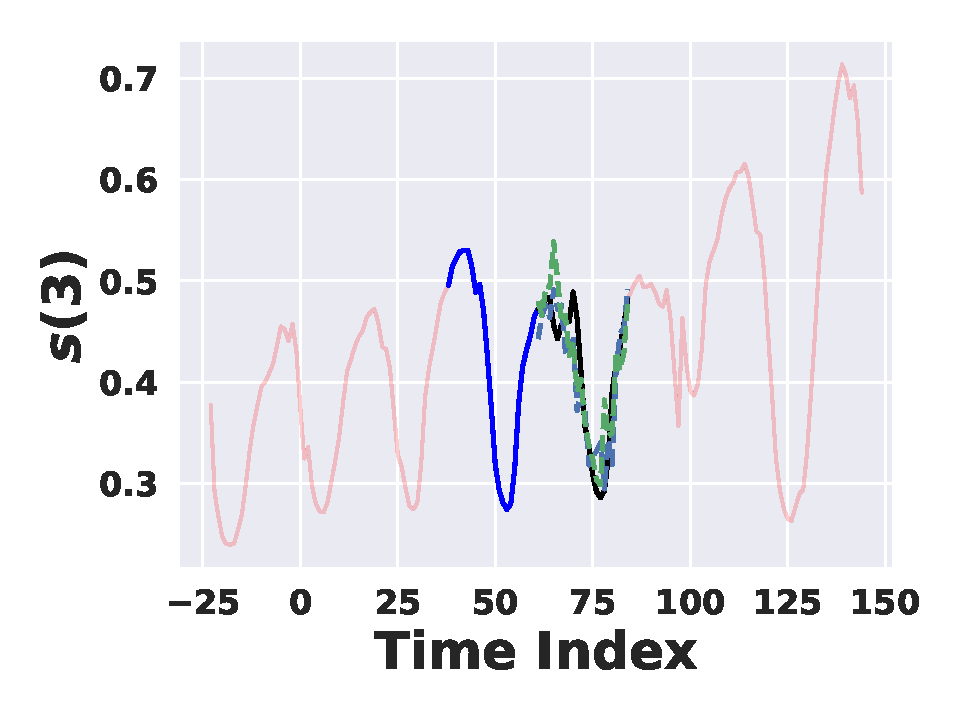
\includegraphics[width=0.4\columnwidth]{figures/appendix/pjm/z_9/forecasts_no_task_aware_sample_1_time_84_signal_3.pdf}}
}

\caption{\textbf{Example forecasts (battery charging).}  Example forecasts at $t=84$ when $Z=4$ (left) and $Z=9$ (right). As before, the predictions are more accurate and smooth when $Z=9$. However, with a smaller bottleneck of $Z=4$ (left), we achieve near-optimal control performance since we capture task-relevant features with a coarse forecast that captures high-level, but salient, trends.}
\label{fig:pjm_forecasts}
\end{center}
\vskip -0.2in
\end{figure}


\textbf{The fully task-aware ($\lambdaforecast = 0$) scheme is good for control but poor for forecasting.} 

Fig. \ref{fig:forecasts_comparison} compares the time-domain forecasts given by task-agnostic/weighted scheme and task-aware scheme. Note that the timeseries starts at $t=-W+1<0$ because $s_{-W+1:0}$ is needed at $t=0$. While the task-agnostic and weighted scheme make reasonable forecasts, the task-aware scheme focuses solely on improving the task-relevant control and imposes no penalties on the forecasting error, leading to poor forecasts. This motivates our weighted approach which balances the control cost and forecasting error.

\textbf{Small $Z$ (e.g., $Z=4$) produces coarse forecasts, which are suitable for good control performance.} 

Fig. \ref{fig:iot_forecasts}, Fig. \ref{fig:cell_forecasts} and Fig. \ref{fig:pjm_forecasts} present the time-domain forecasts with different bottleneck dimensions $Z$ for IoT, taxi scheduling, and battery charging scenarios, respectively. In general, for small $Z$ (e.g., $Z=4$), the task-agnostic scheme makes noisy forecasts which provides room for our weighted scheme to improve the control cost by considering a task-relevant objective. For large $Z$ (e.g., $Z=9$) both the task-agnostic and weighted scheme make smooth forecasts\footnote{The trend is less prominent for the taxi scheduling scenario, because the cell demand itself is rapidly-changing and highly-stochastic.}.

\begin{figure}[ht]
\vskip 0.2in
\begin{center}
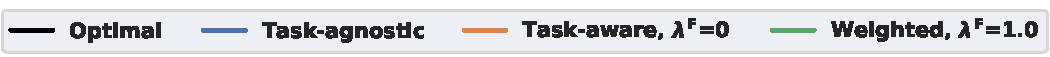
\includegraphics[width=0.8\columnwidth]{figures/evolution_legend.pdf}

\subfigure{
{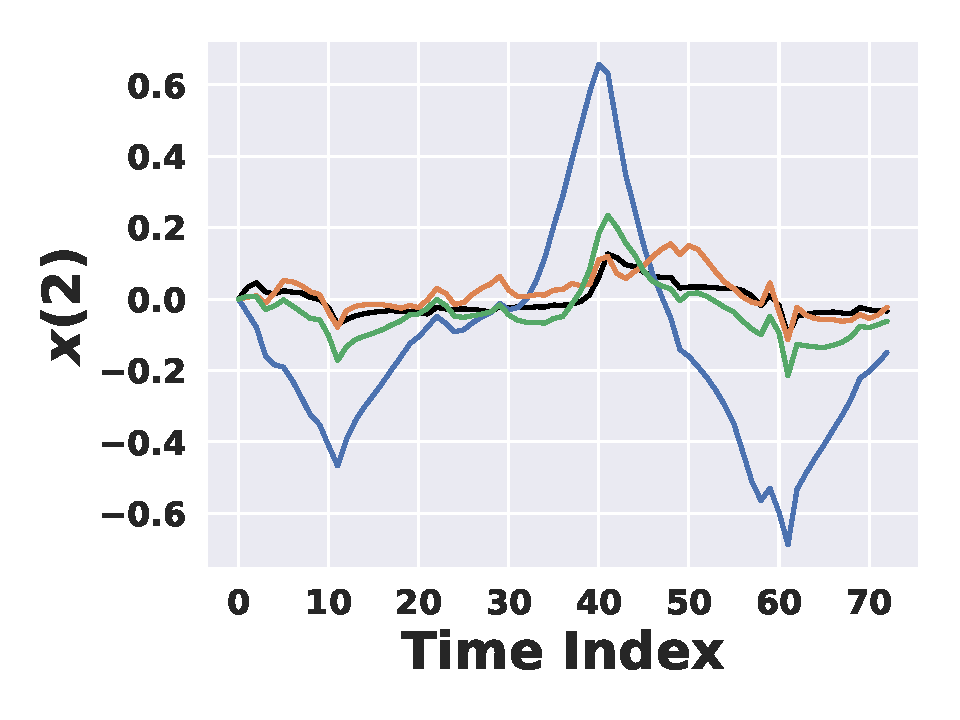
\includegraphics[width=0.31\columnwidth]{figures/appendix/iot/z_4/state_evolution_sample_1_state_2.pdf}}
\label{fig_synthetic_state_evolution}
}
\subfigure{
{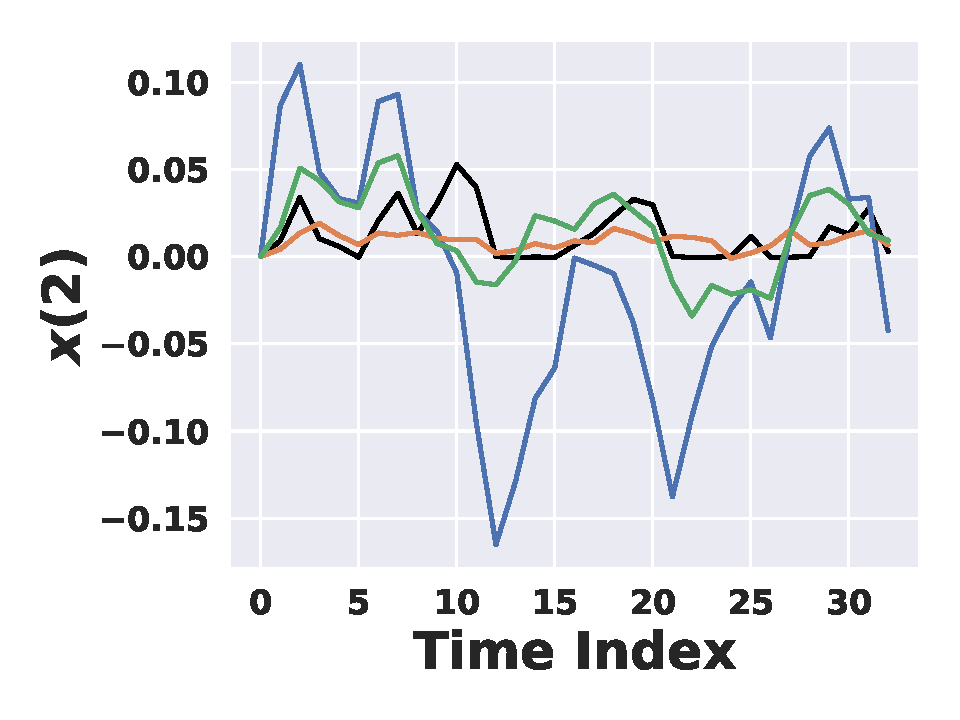
\includegraphics[width=0.31\columnwidth]{figures/appendix/cell/z_4/state_evolution_sample_1_state_2.pdf}}
}
\subfigure{
{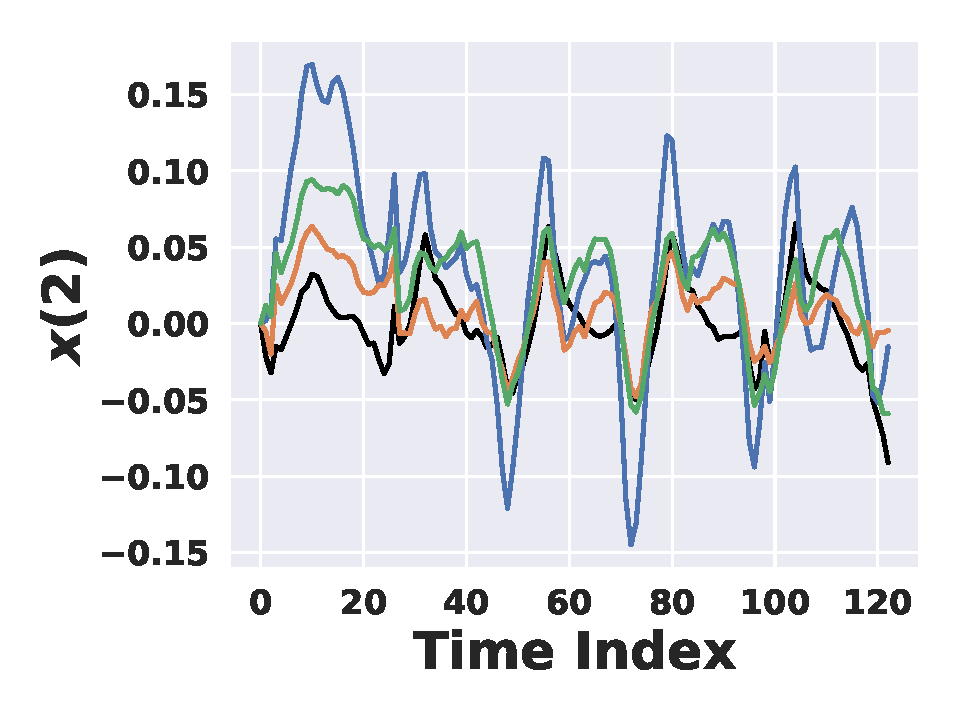
\includegraphics[width=0.31\columnwidth]{figures/appendix/pjm/z_4/state_evolution_sample_1_state_2.pdf}}
\label{fig_synthetic_forecast_errors}
}

\caption{Example evolution of $x(2)$ when $Z = 4$, for IoT (top), taxi scheduling (middle) and battery charging (bottom) scenarios, respectively. Clearly, our co-design approach has state evolutions closer to the unrealizable optimal solution (black) which assumes \textit{perfect} forecasts.}
\label{fig:state_evolution}
\end{center}
\vskip -0.2in
\end{figure}

\textbf{The state evolution of our task-aware/weighted scheme is closer to the optimal trace.} 

Fig. \ref{fig:state_evolution} shows the example state evolution of $x(2)$ for the three scenarios. Importantly, the black trace corresponds to an \textit{unrealizable} baseline with the lowest cost since it assumes \textit{perfect} knowledge of $\bolds$ for the future $H$ steps. We can see that our task-aware and weighted scheme have state evolution traces closer to the optimal trace than the competing task-agnostic scheme. This further explains why task-aware and weighted schemes can yield a near-optimal cost for small $Z$ while the task-agnostic benchmark cannot.
